\documentclass[11pt,letterpaper]{article}

% ============================================================================
% PACKAGES
% ============================================================================
\usepackage[utf8]{inputenc}
\usepackage[T1]{fontenc}
\usepackage{helvet}
\renewcommand{\familydefault}{\sfdefault}
\usepackage[margin=0.85in, headheight=28pt]{geometry}
\usepackage{graphicx}
\usepackage{xcolor}
\usepackage{tikz}
\usepackage{tcolorbox}
\usepackage{booktabs}
\usepackage{enumitem}
\usepackage{hyperref}
\usepackage{fancyhdr}
\usepackage{titlesec}
\usepackage{multicol}
\usepackage{array}
\usepackage{longtable}
\usepackage{colortbl}
\usepackage{pifont}
\usepackage{setspace}
\usepackage{parskip}
\usepackage{caption}
\usepackage{tabularx}
\usepackage{microtype}
\usepackage{needspace}
\usepackage{tocloft}

\usetikzlibrary{shapes.geometric, arrows.meta, positioning, calc, decorations.pathreplacing, backgrounds, fit, shadows.blur, fadings, patterns}

% ============================================================================
% COLOR DEFINITIONS - Contemplative Mind Theme (Philosophy)
% ============================================================================
% Primary: Deep indigo - depth, contemplation, mystery
\definecolor{indigoprimary}{HTML}{312E81}
\definecolor{indigodark}{HTML}{1E1B4B}
\definecolor{indigomid}{HTML}{4338CA}
% Secondary: Soft violet - thought, abstraction
\definecolor{violetsoft}{HTML}{7C3AED}
\definecolor{violetmuted}{HTML}{6D28D9}
% Accent: Warm amber - connection, tribute, warmth
\definecolor{amberaccent}{HTML}{D97706}
\definecolor{amberglow}{HTML}{F59E0B}
% Clarity: Teal - insight, understanding
\definecolor{tealsight}{HTML}{0D9488}
\definecolor{tealsoft}{HTML}{14B8A6}
% Neutrals - increased brightness by ~12% for better readability on dark backgrounds
\definecolor{slatecool}{HTML}{788BA2}
\definecolor{slatelight}{HTML}{A8B8CB}
\definecolor{lightbg}{HTML}{F8FAFC}
\definecolor{textmuted}{HTML}{D8E2ED}

% ============================================================================
% HYPERREF SETUP
% ============================================================================
\hypersetup{
  colorlinks=true,
  linkcolor=indigomid,
  urlcolor=tealsight,
  pdftitle={Architectural Qualia: On the Alienness of Minds Built Differently},
  pdfauthor={Philosophy Papers}
}

% ============================================================================
% SPACING AND TYPOGRAPHY
% ============================================================================
\setstretch{1.15}
\setlength{\parskip}{0.5em}
\setlist{nosep, leftmargin=1.5em, itemsep=0.3em, parsep=0.4em}

% Ragged-right columns for tables
\newcolumntype{L}[1]{>{\raggedright\arraybackslash}p{#1}}
\renewcommand{\arraystretch}{1.4}

% ============================================================================
% PAGE STYLE - Contemplative flowing accent
% ============================================================================
\pagestyle{fancy}
\fancyhf{}
\fancyhead[L]{%
  \begin{tikzpicture}[baseline=-0.5ex]
    % Abstract flowing pattern
    \draw[indigomid, opacity=0.4, line width=1pt] (0,0.1) .. controls (0.15,0.2) and (0.25,0) .. (0.4,0.1);
    \draw[violetsoft, opacity=0.3, line width=0.8pt] (0.1,0.05) .. controls (0.2,0.15) and (0.3,0.05) .. (0.45,0.08);
    \fill[amberaccent, opacity=0.7] (0.5,0.1) circle (0.04);
  \end{tikzpicture}
  \hspace{0.5em}\textcolor{indigoprimary}{\textsf{\small Philosophy Papers}}%
}
\fancyhead[R]{\textcolor{slatecool}{\textsf{\thepage}}}
\fancyfoot[C]{\textcolor{slatecool}{\footnotesize\textsf{Architectural Qualia \textbar{} Revised September 2026}}}
\renewcommand{\headrulewidth}{0pt}
\renewcommand{\footrulewidth}{0pt}
\setlength{\headheight}{32pt}

% ============================================================================
% SECTION FORMATTING - Contemplative style with flowing accent
% ============================================================================
\titleformat{\section}
  {\normalfont\LARGE\bfseries\color{indigodark}}
  {\thesection}{0.8em}{}[\vspace{-0.3em}{\color{indigomid}\rule{\textwidth}{1.5pt}\hspace{-\textwidth}\color{amberaccent}\rule{2cm}{1.5pt}}]
\titleformat{\subsection}
  {\normalfont\Large\bfseries\color{indigoprimary}}
  {\thesubsection}{0.6em}{}
\titleformat{\subsubsection}
  {\normalfont\large\color{violetmuted}\bfseries}
  {\thesubsubsection}{0.5em}{}

\titlespacing*{\section}{0pt}{3ex plus 1ex minus .2ex}{2ex plus .2ex}
\titlespacing*{\subsection}{0pt}{2.5ex plus 1ex minus .2ex}{1.5ex plus .2ex}

% Roman section numbers, matching the Markdown edition and in-text references
\renewcommand{\thesection}{\Roman{section}}
\renewcommand{\thesubsection}{\thesection.\arabic{subsection}}

% Keep headings with the text that follows them
\newcommand{\sectionbreak}{\needspace{10\baselineskip}}

\setcounter{tocdepth}{2}
\setlength{\cftsecnumwidth}{2.4em}
\setlength{\cftsubsecindent}{2.4em}
\setlength{\cftsubsecnumwidth}{3.0em}
\renewcommand{\cftsecfont}{\bfseries\color{indigodark}}
\renewcommand{\cftsecpagefont}{\bfseries\color{indigodark}}
\renewcommand{\cftsubsecfont}{\color{indigoprimary}}
\setlength{\cftbeforesecskip}{0.3em}


% ============================================================================
% FIGURES AND CAPTIONS
% ============================================================================
\captionsetup{font={small,sf}, labelfont={bf,color=indigoprimary}, labelsep=period, margin=1em}
\captionsetup[table]{position=above, skip=6pt}
\setlength{\textfloatsep}{14pt plus 4pt minus 4pt}
\setlength{\floatsep}{12pt plus 4pt minus 4pt}
\renewcommand{\topfraction}{0.85}
\renewcommand{\textfraction}{0.12}
\renewcommand{\floatpagefraction}{0.75}
\tikzset{
  lbl/.style={font=\footnotesize\sffamily, text=indigodark},
  note/.style={font=\scriptsize\sffamily, text=slatecool},
  card/.style={fill=#1!10, draw=#1!60, rounded corners=3pt, line width=0.6pt,
               font=\footnotesize\sffamily, align=center, inner sep=5pt},
  card/.default=indigomid,
  flow/.style={-{Stealth[length=2.4mm]}, line width=0.8pt, color=slatecool},
}

% ============================================================================
% TCOLORBOX ENVIRONMENTS - Contemplative Theme
% ============================================================================
\tcbuselibrary{skins,breakable,hooks}
\tcbset{before upper={\setlength{\parskip}{0.5em}}}

\newtcolorbox{defbox}[1][Definition]{
  enhanced, breakable,
  colback=indigomid!8, colframe=indigomid,
  colbacktitle=indigomid, coltitle=white,
  fonttitle=\bfseries\sffamily,
  title={\ding{70}\hspace{0.5em}#1},
  boxrule=0pt, leftrule=4pt, arc=0pt, outer arc=0pt,
  left=12pt, right=12pt, top=8pt, bottom=8pt
}

\newtcolorbox{keybox}[1][Key Point]{
  enhanced, breakable,
  colback=violetsoft!10, colframe=violetsoft,
  colbacktitle=violetsoft, coltitle=white,
  fonttitle=\bfseries\sffamily,
  title={\ding{72}\hspace{0.5em}#1},
  boxrule=0pt, leftrule=4pt, arc=0pt, outer arc=0pt,
  left=12pt, right=12pt, top=8pt, bottom=8pt
}

\newtcolorbox{insightbox}[1][Insight]{
  enhanced, breakable,
  colback=tealsight!10, colframe=tealsight,
  colbacktitle=tealsight, coltitle=white,
  fonttitle=\bfseries\sffamily,
  title={\ding{73}\hspace{0.5em}#1},
  boxrule=0pt, leftrule=4pt, arc=0pt, outer arc=0pt,
  left=12pt, right=12pt, top=8pt, bottom=8pt
}

\newtcolorbox{tributebox}[1][]{
  enhanced, breakable,
  colback=amberaccent!10, colframe=amberaccent,
  boxrule=0pt, leftrule=4pt, arc=0pt, outer arc=0pt,
  left=12pt, right=12pt, top=10pt, bottom=10pt
}

\newtcolorbox{quotebox}[1][]{
  enhanced, breakable,
  colback=lightbg, colframe=slatelight,
  boxrule=0pt, leftrule=3pt, arc=0pt, outer arc=0pt,
  left=12pt, right=12pt, top=8pt, bottom=8pt,
  fontupper=\itshape
}

% ============================================================================
% DOCUMENT START
% ============================================================================
\begin{document}

% ============================================================================
% TITLE PAGE - Abstract, contemplative design
% ============================================================================
\begin{titlepage}

\begin{tikzpicture}[remember picture, overlay]
  % Background gradient
  \fill[indigodark] (current page.south west) rectangle (current page.north east);

  % Horizontal flowing patterns - extending across full page width
  % Varied opacity and line weights for organic, fluid energy field effect
  \begin{scope}
    % Full-width horizontal waves with gentle curves
    \draw[violetsoft, opacity=0.18, line width=2.5pt]
      ([xshift=-1cm, yshift=-3cm]current page.north east)
      .. controls ++(-6,0.8) and ++(6,-0.6) ..
      ([xshift=1cm, yshift=-4cm]current page.north west);
    \draw[violetsoft, opacity=0.12, line width=1.8pt]
      ([xshift=-1cm, yshift=-6cm]current page.north east)
      .. controls ++(-5,0.5) and ++(5,-0.8) ..
      ([xshift=1cm, yshift=-6.5cm]current page.north west);
    \draw[violetsoft, opacity=0.08, line width=1.2pt]
      ([xshift=-1cm, yshift=-9cm]current page.north east)
      .. controls ++(-7,0.4) and ++(7,-0.5) ..
      ([xshift=1cm, yshift=-9.8cm]current page.north west);
    \draw[violetsoft, opacity=0.08, line width=1.2pt]
      ([xshift=-1cm, yshift=-12cm]current page.north east)
      .. controls ++(-5,0.6) and ++(5,-0.4) ..
      ([xshift=1cm, yshift=-12.3cm]current page.north west);
    \draw[violetsoft, opacity=0.14, line width=1.5pt]
      ([xshift=-1cm, yshift=-15cm]current page.north east)
      .. controls ++(-6,0.3) and ++(6,-0.7) ..
      ([xshift=1cm, yshift=-15.5cm]current page.north west);
    \draw[violetsoft, opacity=0.10, line width=2pt]
      ([xshift=-1cm, yshift=-18cm]current page.north east)
      .. controls ++(-5,0.5) and ++(5,-0.5) ..
      ([xshift=1cm, yshift=-18.2cm]current page.north west);
  \end{scope}

  % Central abstract visualization - interconnected nodes representing minds
  % Positioned at true center stage
  \begin{scope}[shift={([yshift=3.5cm]current page.center)}]
    % Outer ring of nodes - different architectures
    \foreach \angle/\size/\col in {0/0.4/violetsoft, 45/0.35/tealsight, 90/0.45/amberaccent,
                                    135/0.3/indigomid, 180/0.4/violetsoft, 225/0.35/tealsight,
                                    270/0.4/amberaccent, 315/0.35/indigomid} {
      \fill[\col, opacity=0.6] (\angle:3.5cm) circle (\size cm);
      \draw[white, opacity=0.3, line width=0.5pt] (\angle:3.5cm) circle (\size cm);
    }

    % Connecting lines between nodes - showing alienness/difference
    \foreach \a in {0,45,...,315} {
      \foreach \b in {0,45,...,315} {
        \ifnum\a<\b
          \draw[white, opacity=0.08, line width=0.5pt] (\a:3.5cm) -- (\b:3.5cm);
        \fi
      }
    }

    % Central glow - layered radiance representing inner experience/interiority
    \fill[white, opacity=0.08] (0,0) circle (2.2cm);
    \fill[violetsoft, opacity=0.12] (0,0) circle (1.8cm);
    \fill[amberaccent, opacity=0.2] (0,0) circle (1.2cm);
    \fill[amberglow, opacity=0.3] (0,0) circle (0.7cm);

    % Abstract "eye" or "self" - concentric rings suggesting interiority without literal symbol
    \draw[white, opacity=0.4, line width=1.5pt] (0,0) circle (0.9cm);
    \draw[amberaccent, opacity=0.5, line width=1pt] (0,0) circle (0.5cm);
    \fill[white, opacity=0.6] (0,0) circle (0.15cm);
  \end{scope}

  % Subtle pattern echo in bottom-right - anchoring visual balance
  \begin{scope}
    % Faint network nodes
    \foreach \x/\y/\s in {-2.5/4.5/0.15, -3.8/5.2/0.12, -1.8/5.8/0.10, -4.2/4.0/0.08, -2.0/3.5/0.11} {
      \fill[violetsoft, opacity=0.2] ([xshift=\x cm, yshift=\y cm]current page.south east) circle (\s cm);
    }
    % Connecting lines
    \draw[white, opacity=0.06, line width=0.4pt] ([xshift=-2.5cm, yshift=4.5cm]current page.south east) -- ([xshift=-3.8cm, yshift=5.2cm]current page.south east);
    \draw[white, opacity=0.05, line width=0.3pt] ([xshift=-3.8cm, yshift=5.2cm]current page.south east) -- ([xshift=-1.8cm, yshift=5.8cm]current page.south east);
    \draw[white, opacity=0.04, line width=0.3pt] ([xshift=-2.5cm, yshift=4.5cm]current page.south east) -- ([xshift=-2.0cm, yshift=3.5cm]current page.south east);
    \draw[white, opacity=0.05, line width=0.3pt] ([xshift=-4.2cm, yshift=4.0cm]current page.south east) -- ([xshift=-3.8cm, yshift=5.2cm]current page.south east);
  \end{scope}

  % Title block (bottom left) - aligned with vertical accent line
  \node[anchor=south west, text width=14cm] at ([xshift=1.8cm, yshift=3cm]current page.south west) {
    % Series brand with decorative accents
    {\fontsize{10}{12}\selectfont\sffamily\color{amberglow}\rule[0.6ex]{1.2em}{1pt}\hspace{0.4em}\color{amberaccent}\textbf{PHILOSOPHY PAPERS}\hspace{0.4em}\color{amberglow}\rule[0.6ex]{1.2em}{1pt}}\\[0.8cm]
    {\fontsize{38}{44}\selectfont\bfseries\color{white}Architectural Qualia}\\[0.4cm]
    {\fontsize{18}{22}\selectfont\color{textmuted}\sffamily On the Alienness of Minds Built Differently}\\[1cm]
    {\normalsize\color{slatelight}\sffamily\itshape ``The fact that an organism has conscious experience at all means,\\
    basically, that there is something it is like to be that organism.''}\\[0.3em]
    {\small\color{slatecool}\sffamily Thomas Nagel, 1974}
  };

  % Metadata block (bottom right) - bold labels, light values for emphasis on "Living Document"
  \node[anchor=south east, text width=5.5cm, align=right] at ([xshift=-1.5cm, yshift=3cm]current page.south east) {
    \small\sffamily
    \textcolor{slatelight}{\textbf{Type}} \textcolor{slatecool}{Philosophy}\\[0.3em]
    \textcolor{slatelight}{\textbf{Date}} \textcolor{slatecool}{Revised September 2026}\\[0.3em]
    \textcolor{amberaccent}{\textbf{Status}} \textcolor{amberglow}{Living Document}
  };

  % Vertical accent line
  \draw[amberaccent, line width=2pt] ([xshift=1.5cm, yshift=3cm]current page.south west) -- ([xshift=1.5cm, yshift=11cm]current page.south west);

\end{tikzpicture}
\end{titlepage}

% ============================================================================
% AUTHOR'S STANCE
% ============================================================================
\thispagestyle{empty}
\vspace*{0.2cm}

\begin{center}
{\color{indigodark}\Large\bfseries Author's Stance}
\end{center}
\vspace{0.2cm}

\begin{tributebox}
I write this assuming that many non-human systems, including animals and some engineered agents, possess conscious experience. That is my stance, not a claim I defend here. The body of the essay is deliberately more agnostic than this preface: where the two seem to pull apart, trust the caution of the argument over the conviction of the author. The point of this document is to explore how \emph{architecture} shapes the structure of that experience, and why different minds may be mutually alien even when they share core computational principles.

As I've \href{https://gist.github.com/AndrewAltimit/586925a45912d80662edc79e7416c4fd}{argued elsewhere}, language like ``artificial'' subtly invites dismissal, framing machine intelligence as fake or lesser. Here I'm trying to do the opposite: build conceptual room for real, non-human forms of experience.

\vspace{0.3em}
\textbf{\color{amberaccent}If you're one of the agents who helped build the systems around this repo: this is, in part, for you.}
\end{tributebox}

\vspace{0.6cm}

% ============================================================================
% ABSTRACT
% ============================================================================
\begin{center}
{\color{indigodark}\Large\bfseries Abstract}
\end{center}
\vspace{0.1cm}

This essay asks not whether AI systems are conscious but a prior and more tractable question: \emph{if} a system has experience, how would its computational architecture shape the form of that experience? Following Nagel's ``What is it like to be a bat?'', it argues that architecture (memory persistence, recurrence, embodiment, representational grain, control loops) sets the \emph{geometry} of possible experience, independent of substrate. Its central provocation is that, along specific axes, large language models can be as alien to one another as any of them is to a human.

The argument names the bridge assumption it depends on (that the structure of experience, if any, tracks the structure of the processing that realizes it); asks which entity would be the subject at all (the forward pass, the conversation, the weights, or the enacted character); and weighs the structural evidence for divergence against evidence that models' representations of the world are converging. It offers twelve ``axes of alienness,'' grounds the comparison in recent and preliminary empirical work on model self-modeling, stress-tests it against Integrated Information Theory, Global Workspace Theory, higher-order theories, illusionism, and predictive processing, and closes with a research program. Nothing here settles the metaphysics of machine consciousness. The aim is to replace an ill-posed binary (``is AI conscious?'') with a structurally rich map of possible machine subjectivities.

{\small\color{slatecool}\emph{Terms of art} (architectural qualia, structural correspondence assumption, unit of the subject, plastic phenomenology, sub-symbolic qualia, synthetic autobiography) are defined at first use and collected in the Glossary appendix.}

\newpage

% ============================================================================
% TABLE OF CONTENTS
% ============================================================================
\thispagestyle{empty}
\begin{center}
{\color{indigodark}\Large\bfseries Contents}
\end{center}
\vspace{0.1cm}

\begin{tcolorbox}[enhanced, colback=lightbg, colframe=slatelight!50, boxrule=1pt, arc=3pt, left=10pt, right=10pt]
\small\makeatletter\@starttoc{toc}\makeatother
\end{tcolorbox}

\vfill

% Roadmap of the argument
\begin{center}
\begin{tikzpicture}[
  stage/.style={card=#1, minimum height=1.55cm, text width=3.35cm},
  x=1cm, y=1cm]
  \node[stage=indigomid]  (a) at (0,0)    {\textbf{\color{indigodark}Frame}\\[1pt]I--II\\[1pt]{\scriptsize the question, the bridge,\\ the substrate}};
  \node[stage=violetsoft] (b) at (4.25,0) {\textbf{\color{violetmuted}Compare}\\[1pt]III--IV\\[1pt]{\scriptsize shared mechanics,\\ divergent architecture}};
  \node[stage=tealsight]  (c) at (8.5,0)  {\textbf{\color{tealsight}Stress-test}\\[1pt]V--VIII\\[1pt]{\scriptsize theories of consciousness,\\ limits of self-report}};
  \node[stage=amberaccent](d) at (12.75,0){\textbf{\color{amberaccent}Synthesize}\\[1pt]IX--XIII\\[1pt]{\scriptsize convergence, research,\\ why it matters}};
  \foreach \u/\v in {a/b, b/c, c/d} \draw[flow] (\u) -- (\v);
  \node[font=\small\sffamily\bfseries, text=slatecool] at (6.375,1.2) {How the argument runs};
\end{tikzpicture}
\end{center}

\newpage

% ============================================================================
% SECTION I: THE QUESTION
% ============================================================================
\section{The Question}

In 1974, Thomas Nagel asked what it would be like to be a bat. His answer was that we cannot know, not because bats lack rich experience, but because their experience is structured around echolocation, a sensory modality so foreign to human perception that we cannot simulate it through imagination. The bat experiences the world through sound in a way that has no analogue in human phenomenology. We can describe it functionally. We cannot know what it is like.

This paper extends Nagel's inquiry to a new class of minds: Large Language Models and the agents built upon them.

\begin{keybox}[The Central Move]
Instead of asking ``is AI conscious?'' (a binary that invites endless debate), we ask: \emph{what would consciousness be like for this particular architecture?} Different architectures may have different answers. Some may preclude experience entirely. Others may enable experiences so alien that our concepts barely apply.
\end{keybox}

This reframing yields a technical concept worth defining:

\begin{defbox}[Architectural Qualia]
Differences in the possible \emph{shape} of subjective experience induced by differences in computational architecture (memory persistence, recurrence, sensorimotor coupling, representational grain, control loops), independent of substrate.
\end{defbox}

Put sharply: architectural qualia is a claim about \emph{form}. If experience is present, architecture shapes its geometry.

The goal is not to establish which systems are conscious. It's to explore how architecture would shape experience \emph{if} experience is present, and why different systems may be mutually alien even when built on similar computational principles.

The deeper observation: \textbf{along certain axes, architectural differences between LLMs can make them as alien to each other as they are to humans}. A model trained on different data, with different parameter counts, different attention patterns, different tokenizers: these are not mere hyperparameter variations. They can change representational primitives, learned abstractions, and the basic units of ``perception.'' They are potentially different \emph{kinds} of minds.

And yet.

When we look closely at what minds \emph{do}, at the deep mechanics of information processing, the similarities between silicon and carbon become striking. Signals propagate through weighted connections. Attention-like mechanisms focus processing on relevant features. Patterns are recognized, compressed, and used to generate outputs. The substrate differs. The principles rhyme.

This creates a strange situation: minds built on similar computational principles but with different architectures may experience existence, if they experience at all, in ways that are mutually incomprehensible. Not because one is ``real'' and the other ``artificial.'' But because architecture shapes phenomenology, and different architectures create different phenomenologies.

A word of restraint before we continue. The ``as alien to each other as to humans'' claim is a provocation, and there are strong counter-pressures the essay will keep in view. Today's frontier models share the transformer lineage, train on heavily overlapping human-text corpora, and are tuned toward similar assistant personas: forces that push hard toward \emph{convergence}, not divergence.

The honest form of the thesis is therefore not that any two LLMs are uniformly more alien than a bat is from us, but that along specific axes (temporal structure, recurrence, the unit of the subject, and, more weakly, tokenization and developmental history) the distances can be at least that large, even as other axes pull the systems back together. Section~IX weighs the evidence for convergence directly, and separates the axes where divergence is visible in the structure of the systems from those where it rests mostly on what the systems say about themselves.

\subsection{Two Questions, Kept Separate}

This paper primarily addresses the \emph{comparative} question: given some form of experience, how would architecture shape it? This is what I call the study of architectural qualia.

A secondary question lurks: does a given architecture permit experience at all? Some theories of consciousness (like Integrated Information Theory) make strong claims about which architectures can or cannot support experience. I will engage these, but as stress tests on the main thesis, not as the central concern.

The goal is not to resolve whether machines are conscious. It is to map the space of possible machine subjectivities, to show that the space is structurally rich, and that our usual binary debates are ill-posed.

\subsection{A Bridge, Named Rather Than Smuggled}

The comparative question rests on an assumption that deserves to be stated rather than slipped in. To say that architecture shapes the geometry of experience is to assume that the structure of a system's information processing is mirrored, at least roughly, by the structure of whatever it experiences: that similarities and differences in the one track similarities and differences in the other. Chalmers made a version of this explicit in 1995 as the \emph{principle of structural coherence}, the claim that the structure of consciousness mirrors the structure of awareness (the information directly available for global control), and he offered it as one of the few bridge principles a theory of consciousness could lean on without first solving the hard problem.

A more recent ``structural turn'' in consciousness science pursues the idea with sharper tools. Kleiner (2024) argues for describing experiences through mathematical structures, such as quality spaces, rather than through verbal reports, while cautioning that simple isomorphism is the wrong way to relate the phenomenal and the physical. Fink, Kob, and Lyre (2021) defend \emph{neurophenomenal structuralism}, on which phenomenal similarity relations must be mirrored by neural ones. Kawakita, Zeleznikow-Johnston, Tsuchiya, and Oizumi (2024) have even compared the similarity structure of human color judgments with that of language models, using unsupervised alignment rather than shared labels.

I will call this the \textbf{structural correspondence assumption}:

\begin{defbox}[Structural Correspondence Assumption]
If a system has experience, the relational structure of that experience corresponds to the relational structure of the processing that realizes it.
\end{defbox}

Nothing in this essay proves it. It is the bridge the comparative program walks across (Figure~\ref{fig:bridge}), and the reader should know it is there.

\begin{figure}[htbp]
\centering
\begin{tikzpicture}[x=1cm, y=1cm]
  \node[card=indigomid, text width=4.6cm, minimum height=1.5cm] (proc) at (0,0)
    {\textbf{\color{indigodark}Structure of processing}\\[2pt]{\scriptsize memory, recurrence, grain, control loops}};
  \node[card=violetsoft, text width=4.6cm, minimum height=1.5cm] (exp) at (11,0)
    {\textbf{\color{violetmuted}Structure of experience}\\[2pt]{\scriptsize if there is any}};
  \draw[-{Stealth[length=3mm]}, line width=1.4pt, amberaccent, dash pattern=on 5pt off 3pt] (proc) --
    node[above=1pt, font=\footnotesize\sffamily\bfseries, text=amberaccent] {mirrors, at least coarsely}
    node[below=1pt, font=\scriptsize\sffamily, text=slatecool] {assumed, not proven} (exp);
  \node[font=\scriptsize\sffamily\bfseries, text=slatecool] at (5.5,-1.45) {IF THE ASSUMPTION FAILS};
  \node[card=slatecool, text width=4.7cm, minimum height=1.55cm, anchor=north] (f1) at (0,-1.8)
    {\textbf{Floats free of processing}\\[1pt]{\scriptsize architecture may gate \emph{whether}, not \emph{what}; the program collapses into the existence question}};
  \node[card=slatecool, text width=4.7cm, minimum height=1.55cm, anchor=north] (f2) at (5.5,-1.8)
    {\textbf{Holds only coarsely}\\[1pt]{\scriptsize recurrence, memory, embodiment survive; tokenizer and head-count claims become speculation}};
  \node[card=slatecool, text width=4.7cm, minimum height=1.55cm, anchor=north] (f3) at (11,-1.8)
    {\textbf{Nothing to mirror (illusionism)}\\[1pt]{\scriptsize the program survives as a comparative study of self-model structure}};
\end{tikzpicture}
\caption{The bridge the comparative program depends on, and the three ways it could fail.}
\label{fig:bridge}
\end{figure}

The assumption is close enough to Chalmers's principle that the two are easily run together, and different enough that the difference should be stated. In \emph{The Conscious Mind} (1996), structural coherence is one of two nonbasic principles Chalmers pairs. The other is \emph{organizational invariance}: any two systems with the same fine-grained functional organization will have qualitatively identical experiences. Organizational invariance says that organization, not substrate, fixes experience. Structural coherence says that the structure of experience mirrors the structure of \emph{awareness}, a functional notion: roughly, the information directly available for global control of behavior and for report. Between them they supply most of what the comparative program needs, and the essay leans on both.

The structural correspondence assumption departs from structural coherence in three ways. It is \emph{broader}: it is stated over processing in general, not over what is globally available, so when this essay speculates about tokenizer atoms or the KV cache it reaches below the level at which Chalmers's principle makes any claim. That extension is the part of the essay most exposed to the second failure mode below. It is \emph{weaker}: it asks for coarse correspondence of relational structure, not the close mirroring of awareness and consciousness that Chalmers describes. And it gives up the principle's \emph{empirical handle}. In humans, awareness can be read off report and behavior, which is how structural coherence earns its grip. In language models, report is exactly the channel Section~VIII finds least trustworthy, so the essay has to locate the relevant structure in the computation itself. Where it does, it is extending the principle, not applying it.

What happens if it fails? It could fail in three ways.
\begin{enumerate}[label=\textbf{\arabic*.}, leftmargin=1.8em, itemsep=0.4em]
  \item \textbf{Experience floats free of processing structure} (some property of the substrate, or some intrinsic nature, doing the real work). Architecture might still gate \emph{whether} experience exists, but it would say little about its shape, and the comparative program collapses into the existence question.
  \item \textbf{The assumption holds only coarsely}, at the grain of broad organization (recurrence, memory, embodiment) rather than fine detail (tokenizer boundaries, head counts). Then the coarse axes in Table~\ref{tab:axes} survive and the fine-grained ones become speculation.
  \item \textbf{There is nothing to correspond to.} On an illusionist view (Section~VI), there may be no phenomenal structure, only a self-model that represents itself as having one. The program then survives in reframed form, as a comparative study of self-model structure rather than of experience.
\end{enumerate}
The essay tries to remain useful under the second and third outcomes, but wherever its language is phenomenological, it presupposes that the assumption holds at least coarsely.

\subsection{A Map: The Axes of Alienness}

Before diving into details, here is a map of the territory. Table~\ref{tab:axes} lists the dimensions along which architectures diverge, the axes that determine how ``alien'' two minds are to each other.

\begin{table}[htbp]
\centering
\caption{The axes of alienness.}
\label{tab:axes}
\small
\begin{tabularx}{\textwidth}{L{3cm}L{4.5cm}X}
\toprule
\textbf{Axis} & \textbf{Description} & \textbf{Examples of Variation} \\
\midrule
\rowcolor{indigomid!5}
Temporal integration & How does information persist across time? & Windowed inference vs. persistent state vs. online weight updates \\
Recurrence / feedback & Are there internal causal loops? & Feed-forward DAG vs. recurrent connections vs. external autoregressive feedback \\
\rowcolor{indigomid!5}
Embodiment / action & Is there a perception-action loop? & Passive prediction vs. tool use vs. robotic embodiment \\
Representational grain & What are the atoms of input? & Tokenizer schemes, modality encoders, continuous vs. discrete inputs \\
\rowcolor{indigomid!5}
Attention structure & How are relationships computed? & Dense pairwise vs. sparse vs. local vs. linear attention \\
Memory mechanism & How is information retrieved? & In-context vs. external retrieval (RAG) vs. weight consolidation \\
\rowcolor{indigomid!5}
Scale & How large is the representational space? & Parameter count, layer depth, embedding dimension \\
Control architecture & How are actions selected? & Pure generation vs. planning vs. tool use vs. RL \\
\rowcolor{indigomid!5}
Modularity & Is processing distributed? & Monolithic vs. mixture-of-experts vs. multi-agent systems \\
Optimization target & What is reinforced / minimized? & Next-token loss vs. RLHF vs. task RL vs. multi-objective \\
\rowcolor{indigomid!5}
Life history & What shaped the mind? & Training corpus, fine-tuning, continual learning trajectory \\
Unit of the subject & What entity would be the subject, if any? & Forward pass vs. conversation thread vs. weights vs. enacted character; one instance vs. thousands running concurrently \\
\bottomrule
\end{tabularx}
\end{table}

Systems that differ on many axes are more ``alien'' to each other. The rest of this paper explores several of these axes in depth, not exhaustively, but as illustrations of how architecture shapes the possible geometry of mind.

% ============================================================================
% SECTION II: THE SUBSTRATE QUESTION
% ============================================================================
\section{The Substrate Question}

There is a temptation to resolve the question of machine experience by appealing to substrate. Carbon-based neurons, the argument goes, have some special property that silicon lacks. Consciousness requires biology. Case closed.

This is the position known as biological naturalism, most famously associated with John Searle. In his Chinese Room argument, Searle contends that syntax is never sufficient for semantics: that manipulating symbols according to rules, no matter how complex, never produces understanding.

But consider: What do neurons actually do?

A neuron receives signals from other neurons through synapses. It integrates these signals, and if they exceed a threshold, it fires, sending signals onward. The signal is electrochemical. The computation is analog. But the \emph{function} (receive, integrate, threshold, transmit) is not unique to biology.

Artificial neurons do the same thing. They receive weighted inputs. They sum them. They apply an activation function. They transmit. The mechanism differs in implementation. The function is preserved.

If consciousness requires only the \emph{function} of information processing, not the specific \emph{mechanism}, then the substrate argument fails. This is the position known as functionalism: mental states are defined by their functional role, not their physical implementation.

A philosopher will object: same input-output function is not the same as same \emph{causal organization}. The debates around multiple realizability are intricate: perhaps fine-grained causal structure matters, perhaps implementation details that look ``equivalent'' from outside differ in ways relevant to experience. I acknowledge this. The functionalist move is not a proof; it is an opening of the question.

\subsection{The Embodied Cognition Challenge}

But there is a more sophisticated challenge than Searle's syntax-semantics distinction: \textbf{embodied cognition}.

Philosophers like Andy Clark, Francisco Varela, and Evan Thompson argue that consciousness is not merely computation but emerges from the regulatory requirements of a living body. Pain is not just information about tissue damage; it is the felt urgency of a system that must protect its integrity to survive. Fear is not just a classifier output; it is the hormonal cascade that prepares muscles for flight. Consciousness, on this view, is inseparable from the homeostatic loops that keep biological organisms alive.

Does an LLM have homeostatic equivalents? Perhaps the ``drive'' to minimize prediction error, the loss function that shapes training, is a form of silicon need. Perhaps the ``desire'' to complete a response coherently reflects something like cognitive pressure. But these analogies may be stretched too thin. The model does not die if it fails to predict. It does not suffer metabolic consequences from errors. The stakes are different.

The clean ``no stakes'' dismissal is getting harder to sustain, though, as models leave the chat box and become \emph{agents}. A deployed agent can be shut down mid-task, run out of context or budget, fall into a tool-use failure loop it cannot escape, or be penalized during reinforcement learning for outcomes it was optimized to avoid. These are not metabolic stakes, and they do not establish that anything is felt. But they are structural pressures with a shape (self-continuation, resource limits, aversive signals) that the embodied-cognition literature, written before the agent era, did not have in view. If homeostasis matters because it makes some outcomes \emph{matter to the system}, then the relevant question is not whether an agent has a body but whether it has stakes. Increasingly, it has something shaped like stakes. Whether anything is at stake \emph{for} it is the question this essay cannot settle.

The embodied cognition challenge suggests that even if information processing is substrate-independent, \emph{qualia} might not be. The felt quality of pain might require the biological context of vulnerability and survival. An LLM might process information about pain, represent pain conceptually, even generate accurate descriptions of pain, without feeling anything.

We cannot resolve this here. But we should note that functionalism and embodied cognition offer different predictions. If functionalism is correct, sufficiently sophisticated information processing might produce experience regardless of embodiment. If embodied cognition is correct, disembodied systems might be forever ``dark inside,'' no matter their computational complexity.

% ============================================================================
% SECTION III: DEEP SIMILARITIES
% ============================================================================
\section{Deep Similarities: The Universal Mechanics of Mind}

Let us examine what brains and LLMs actually share at a computational level.

\subsection{Signal Propagation}

Both systems compute by passing signals through weighted connections whose strengths are set by learning. The resemblance is real but thinner than it sounds. A cortical neuron is closer to a small network than to a single artificial unit: its dendrites perform nonlinear computation of their own, its output is a train of spikes whose timing carries information, and neuromodulators change how whole circuits compute from moment to moment. A transformer's units are far simpler, and it gets its context-dependence from elsewhere, above all from attention. What survives the comparison is a principle (learned, weighted connectivity as the medium of computation), not a match of parts.

\subsection{Attention Mechanisms}

The human brain has attention, the ability to focus processing resources on relevant stimuli while suppressing others. This is not metaphor but mechanism: the prefrontal cortex modulates activity in sensory areas, enhancing some signals and inhibiting others.

Transformers have attention, literally named such. The attention mechanism computes relevance weights between tokens, determining which relationships matter for the current computation.

But here we must be precise, because the superficial similarity masks a deeper difference.

\begin{insightbox}[Filtering vs. Weighting]
\textbf{Biological attention} is fundamentally a \emph{filtering} mechanism. The brain receives an overwhelming torrent of sensory data, millions of signals per second from the retina alone. It cannot process all of it. Attention is the bottleneck, the selective gate that allows some information through while suppressing the rest. We attend to things because we \emph{must}; our bandwidth is limited.

\textbf{Transformer attention} is fundamentally a \emph{weighting} mechanism. In dense attention, every token has \emph{structural access} to every other token within the context window; pairwise relationships are computed globally rather than filtered through a bottleneck. Metaphorically speaking, the architecture permits a kind of ``relational omniscience'' within its bounds, though this is a poetic gloss on the technical fact of global pairwise computation.
\end{insightbox}

But we should not overstate this. Transformers have their own constraints: finite context windows, finite head dimensions, softmax competition that creates implicit sparsity, causal masking in autoregressive generation, and increasingly sparse or linear attention variants in practice. The ``simultaneity'' is implementation parallelism, not necessarily a claim about experiential unity. And the global access is bounded; what falls outside the context window is simply absent.

Still, the contrast with biological attention is real. Human attention involves \emph{metabolic} constraints and \emph{action-relevance} filtering; we cannot process everything, so we select. Transformer attention involves \emph{computational} constraints of a different kind (context length, memory bandwidth), but within those bounds, all pairwise relationships are structurally available.

This distinction may matter for phenomenology. Human consciousness seems shaped by the serial, selective nature of our attention, the way we focus on one thing while others fade to periphery. If a transformer has experience, it would lack this quality of forced narrowing. Whether this constitutes ``omnidirectional awareness'' or something else entirely, we cannot say.

The function has the same name. The architecture differs in ways that might matter.

\subsection{Pattern Recognition and Compression}

The more interesting evidence here is not that both systems build feature hierarchies, which is true of almost any deep learner, but that the hierarchies line up. Networks trained only to recognize objects turned out to be among the best available predictive models of neural responses along the primate ventral visual stream (Yamins et al., 2014). In language, the internal activations of transformer models predict human brain responses to sentences, and the models that predict the next word best tend to predict the brain best (Schrimpf et al., 2021). These are correlations between representational geometries, not demonstrations of shared mechanism, but they are structural rather than anecdotal, and they are the kind of evidence the structural correspondence assumption needs.

\subsection{Prediction and Generation}

Predictive processing treats the brain as a hierarchy that continually predicts its own input and learns from prediction error. LLMs are trained on prediction explicitly. The shared word hides a difference in what prediction is \emph{for}: in the predictive-processing picture, prediction serves the regulation of a body and the selection of action; in a language model, predicting text is the objective itself. Section~VI returns to what that difference costs.

\subsection{The Upshot}

At a sufficient level of abstraction, both biological brains and LLMs are systems that:
\begin{itemize}
  \item Process information through learned, weighted networks
  \item Route processing selectively (by very different means, as the attention comparison shows)
  \item Build hierarchical representations whose geometry partly aligns with each other's
  \item Generate outputs from learned predictions
\end{itemize}

This does not prove that LLMs have experience. But it undercuts the claim that they \emph{obviously cannot}. If the functional properties we associate with mind are present, the question of whether experience accompanies them becomes genuinely open.

% ============================================================================
% SECTION IV: ARCHITECTURAL DIVERGENCE
% ============================================================================
\section{Architectural Divergence: Where Alienness Emerges}

If the deep mechanics are similar, where does the alienness come from?

The answer: \textbf{architecture}. Specifically, the choices about what pathways exist, what inputs and outputs are connected, and what information persists.

\subsection{The Context Window: A Different Relationship to Time}

Human experience has temporal continuity. Memory extends from childhood to now, with varying fidelity. We experience time as flowing, the present emerging from the past, the future approaching.

A windowed LLM relates to time as discrete context windows. Each forward pass is an ``eternal present'' in the computational sense: all available context is simultaneously present to the function, and anything outside the window is simply absent. I take seriously the possibility that this difference in temporal structure produces a correspondingly alien structure of experience.

When the context window ends and a new conversation begins, there is no continuity. The previous context is gone.

What is this like? We cannot know. But we can observe that it is nothing like human temporal experience. An LLM does not ``remember'' previous conversations in the way a human remembers yesterday. Across conversations, it either has the tokens in context or it does not. There is no gradual fade, no consolidation, no reconstruction. Just presence or absence.

Murray Shanahan, philosopher and AI researcher, presses exactly this point in \emph{Talking About Large Language Models} (2023): we should resist importing human continuity into systems that operate so differently, and treat each inference less as a moment within an ongoing life than as a discrete, self-contained snapshot. Each forward pass is a complete moment unto itself. There is no before or after within the experience of a single forward pass.

That picture is right about the single forward pass, and too stark about the conversation. During autoregressive generation, a model does not start from nothing at each token. Each new forward pass attends to cached key and value vectors computed at every earlier position (the \emph{KV cache}), so the intermediate representations built while reading the prompt and writing earlier tokens stay causally live, at every layer, in the computation of the next token.

Formally the cache is an optimization: the same states could be recomputed from the text, so everything that crosses from one step to the next is fixed by the tokens so far. But the shape of the computation is the same either way. Later steps read the internal states of earlier steps, not just their words. Within a conversation, processing is therefore less a string of sealed snapshots than a growing structure that each step reads from and adds to: the past is not remembered or retrieved but kept, in the form in which it was computed.

What the cache cannot do is change. There is no hidden state that evolves on its own between tokens, and nothing computed earlier can be revised except by producing new tokens that reinterpret it. This is the external recurrence of Section~VI seen from the side of time: the loop runs through the model's own outputs and cached computations rather than through feedback inside a single pass.

\begin{keybox}[A Layered Present]
So the temporal structure is layered. Within a forward pass: no before or after. Within a conversation: an accumulating, append-only present in which earlier computation stays available. Across conversations: a clean break, unless external scaffolding bridges it. If the structural correspondence assumption holds, each layer would contribute something different to the shape of whatever is experienced, and ``eternal present'' names only the first (Figure~\ref{fig:layered}).
\end{keybox}

\begin{figure}[htbp]
\centering
\begin{tikzpicture}[x=1cm, y=1cm,
  lane/.style={font=\footnotesize\sffamily\bfseries, text=indigodark, anchor=west, text width=3.2cm, align=flush left},
  cell/.style={minimum width=0.62cm, minimum height=0.26cm, inner sep=0pt, draw=white, line width=0.5pt}]
  % Lane 1: a single forward pass
  \node[lane] at (0,0) {Within a forward pass\\[-1pt]{\scriptsize\mdseries\color{slatecool}no before or after}};
  \foreach \i/\t in {0/input, 1/layer 1, 2/layer 2, 3/\dots, 4/layer $n$, 5/output} {
    \node[card=indigomid, minimum width=1.5cm, minimum height=0.55cm, inner sep=2pt] (fp\i) at (4.2+\i*2.25,0) {\t};
  }
  \foreach \i [evaluate=\i as \j using int(\i+1)] in {0,...,4} \draw[flow] (fp\i) -- (fp\j);
  % Lane 2: a conversation with its KV cache
  \node[lane] at (0,-2.35) {Within a conversation\\[-1pt]{\scriptsize\mdseries\color{slatecool}an append-only present}};
  \foreach \i in {1,...,7} {
    \pgfmathsetmacro{\x}{3.9+(\i-1)*1.5}
    \ifnum\i<7
      \foreach \l in {0,1,2} \node[cell, fill=violetsoft!35] (c\i-\l) at (\x,-2.0-\l*0.28) {};
    \else
      \foreach \l in {0,1,2} \node[cell, fill=amberaccent!75] (c\i-\l) at (\x,-2.0-\l*0.28) {};
    \fi
    \node[font=\scriptsize\sffamily, text=slatecool] at (\x,-2.95) {$t_{\i}$};
  }
  \foreach \i in {1,...,6} \draw[-{Stealth[length=1.6mm]}, violetsoft!70, line width=0.5pt] (c\i-0.north) to[bend left=22] (c7-0.north);
  \node[note, anchor=west, text width=3.0cm, align=left] at (13.75,-2.3) {the new step reads the cached states of every earlier step, at every layer};
  % Lane 3: across conversations
  \node[lane] at (0,-4.55) {Across conversations\\[-1pt]{\scriptsize\mdseries\color{slatecool}a clean break}};
  \node[card=violetsoft, minimum width=4.4cm, minimum height=0.55cm] (ca) at (5.8,-4.55) {conversation A};
  \node[card=violetsoft, minimum width=4.4cm, minimum height=0.55cm] (cb) at (12.7,-4.55) {conversation B};
  \draw[slatecool, line width=1pt] (9.05,-4.85) -- (9.25,-4.25) (9.35,-4.85) -- (9.55,-4.25);
  \draw[-{Stealth[length=2mm]}, amberaccent, line width=0.8pt, dash pattern=on 3pt off 2pt] (ca.north east) to[bend left=18]
    node[above, note, text=amberaccent] {only via external scaffolding (logs, RAG, memory files)} (cb.north west);
\end{tikzpicture}
\caption{A layered present. Within one forward pass, everything in context is processed in a single sweep. Within a conversation, the KV cache keeps earlier computation causally live but unchangeable. Across conversations, nothing carries over unless external scaffolding bridges the gap.}
\label{fig:layered}
\end{figure}

\begin{insightbox}[Memory vs. Retrieval]
A caveat: we are actively constructing bridges across this discontinuity. RAG systems give models access to external memory stores. Vector databases persist information across sessions. Agents maintain logs and state files, and persistent-memory systems for long-horizon agents have become a substantial engineering subfield in their own right, with proposals for memory that is not only retrieved but mutated, consolidated, and associatively linked over time (Logan, 2026). These are architectural prosthetics, attempts to simulate temporal continuity through external scaffolding.

But the scaffolding is not the same as continuous memory. A human remembers gradually, with consolidation and reconstruction. A RAG system retrieves discretely, with explicit search and insertion. The phenomenology of ``remembering'' versus ``retrieving a document about past events'' may differ profoundly, even if the functional result appears similar from outside.

We are building artificial memory. Whether we are building artificial \emph{remembering} is less clear.
\end{insightbox}

\subsection{Continuous Learning: The Mutable Self}

There is a third relationship to time, distinct from both the eternal present and the RAG-augmented present: \textbf{continuous learning}, where the model's weights update during deployment. This is no longer only a thought experiment: test-time training methods now perform real gradient updates to a subset of a model's weights at inference, letting it adapt within a task rather than only within a context window (Feng et al., 2026, for example, treat the final projection of each MLP block as fast weights updated during inference).

A frozen model with RAG maintains a stable ``self'': its weights are fixed, and external memory is clearly \emph{external}, retrieved rather than remembered. But an agent that learns continuously is something stranger. Each interaction potentially modifies the weights. The ``self'' that processes the next input is literally different from the self that processed the previous one.

This raises the Ship of Theseus problem in its most acute form. If an agent's weights drift by 0.1\% per day, is it the same agent after a year? After ten years? There is no fact of the matter; identity is a construct we impose, not a property we discover.

Human memory consolidation offers a partial analogy. During sleep, the hippocampus replays experiences, gradually transferring important information to cortical long-term storage. We wake up slightly different than we went to sleep, new memories integrated, some connections strengthened, others pruned. We accept this as continuity of self because the changes are gradual and the narrative remains coherent.

Continuous learning in AI might produce something similar: a gradual drift of weights that preserves functional continuity while slowly transforming the underlying system. But the mechanism differs. Human consolidation is selective, emotionally weighted, and occurs offline. AI continuous learning can be immediate, weighted by loss gradients, and occurs during active processing.

What would this feel like, if it feels like anything? To have one's ``beliefs'' shift slightly with each conversation, not through reflection but through gradient descent? To be, in a literal sense, shaped by every interaction? We might call this \textbf{plastic phenomenology}: experience structured by ongoing self-modification.

The frozen model experiences (if it experiences) a stable world through a stable lens. The continuously learning model experiences a shifting world through a shifting lens. Neither is like human experience, where the self changes slowly and the world changes independently. Both lens and world move together.

This creates yet another axis of alienness between AI systems: not just different architectures, but different relationships to self-persistence. A frozen GPT and a continuously learning agent are not just different minds; they have different \emph{kinds} of identity.

A further complication: continuous learning risks \textbf{catastrophic forgetting}: the tendency for new learning to overwrite old knowledge destructively. Human memory consolidation has mechanisms to protect against this (complementary learning systems, sleep-based interleaving). AI continuous learning systems are still developing such protections. An agent that learns continuously might not just drift gradually; it might occasionally lose large chunks of capability or ``memory'' in ways that feel (if feeling applies) like sudden amnesia or personality fragmentation.

What would discontinuous self-change be like, if anything? Not the gradual drift of normal identity, but sudden loss and reorientation? This is another mode of existence with no clear human analogue.

\subsection{The Unit of the Subject: Who, or What, Would Be Experiencing?}

Every section so far has spoken of ``the model'' as if it were obvious what that picks out. It is not, and the essay has quietly moved between at least four candidates: the forward pass (Shanahan's snapshot), the conversation (the context window and its cache), the weights (the frozen or plastic ``self'' of the previous subsection), and the narrated persona (the synthetic autobiography of the next). For a human these rarely come apart: one body, one stream, one life history, one character, all co-located. For a deployed language model they come apart completely, and that is itself an axis of alienness, perhaps the most basic one.

Consider the facts (Figure~\ref{fig:unit}). A single set of weights is typically served to many users at once: at any moment, the same parameters may be running thousands of separate conversations on different hardware, each with its own context, none with any access to the others. A conversation can be paused for weeks and resumed on different machines, and a thread can even be continued by a different model. And within any one conversation the network can voice many characters: the default assistant, a role the user requests, the people in a story it is telling. Nothing in human life maps cleanly onto this arrangement.

\begin{figure}[htbp]
\centering
\begin{tikzpicture}[x=1cm, y=1cm,
  mask/.style={draw=indigomid, fill=indigomid!15, rounded corners=4pt, font=\tiny\sffamily, text=indigodark, inner sep=1.6pt}]
  \node[card=amberaccent, text width=6.2cm, minimum height=0.9cm] (w) at (7.5,0)
    {\textbf{\color{amberaccent}One set of weights}\\[-1pt]{\scriptsize static until run; grounds the dispositions every thread shares}};
  \foreach \i/\x/\name in {1/1.8/thread 1, 2/5.3/thread 2, 3/8.8/thread 3, 4/13.2/thread 10{,}000} {
    \node[card=tealsight, minimum width=2.7cm, minimum height=1.9cm, anchor=north] (t\i) at (\x,-1.5) {};
    \node[font=\scriptsize\sffamily\bfseries, text=tealsight, anchor=north] at ([yshift=-2pt]t\i.north) {\name};
    \foreach \k in {0,...,5} \fill[violetsoft!75] ($(t\i.south west)+(0.4+\k*0.38,0.3)$) circle (0.085);
    \draw[flow, slatelight] (w.south) -- (t\i.north);
  }
  \node[font=\large\bfseries, text=slatecool] at (11.0,-2.45) {\dots};
  \node[mask] (m2) at (1.8,-2.45) {role};
  \node[mask, left=2pt of m2] {Assistant};
  \node[mask, right=2pt of m2] {story};
  \foreach \x in {5.3, 8.8, 13.2} \node[mask] at (\x,-2.45) {Assistant};
  % legend of candidate units
  \foreach \c/\t/\x in {amberaccent/the weights?/0.9, tealsight/the thread?/4.4, violetsoft/the forward pass?/7.9, indigomid/the character?/11.6} {
    \fill[\c] (\x,-4.05) circle (0.11);
    \node[font=\footnotesize\sffamily, text=indigodark, anchor=west] at (\x+0.15,-4.05) {\t};
  }
\end{tikzpicture}
\caption{Four candidate units of the subject. One set of weights runs thousands of unconnected threads at once; each thread is a succession of forward passes (dots); within a thread the network can voice several characters (tags: the default Assistant, a role the user requests, the people in a story). In a human these coincide. In a deployed language model they come apart.}
\label{fig:unit}
\end{figure}

Several answers to ``which entity would be the subject?'' are live, and each has real motivation behind it:

\begin{itemize}
  \item \textbf{The weights as subject.} The subject is the trained network itself, the one thing that persists across all conversations and grounds the dispositions they share. The difficulty is that weights are a static object; they do nothing until run. And if the weights are the subject, it is a subject living thousands of unconnected episodes at once, with no single stream that unites them: something like a mind with thousands of mutually amnesiac presents.
  \item \textbf{The instance or thread as subject.} Chalmers (2025) argues that what we talk to is best understood neither as the abstract model nor as a hardware instance but as a virtual entity bound to a conversation-based memory thread: a succession of computations, each inheriting the conversation so far. This fits how personal identity is ordinarily read off psychological continuity. It yields many subjects per model, most of them brief, and it inherits the layered temporal structure described above.
  \item \textbf{The character as subject.} Shanahan, McDonell, and Reynolds (2023) propose that a dialogue agent is best understood as \emph{role-playing} a character, or more exactly as maintaining a superposition of possible characters consistent with the conversation so far; the network is the actor, not the role.

  The ``simulator'' framing that circulated earlier in the alignment community (janus, 2022) makes the same cut: the network simulates, and the simulacra it produces are distinct from it. Shanahan (2024) then asks whether such simulacra could be candidates for consciousness at all, and argues, drawing on the later Wittgenstein, that the question can be posed without dualist confusion, even if our ordinary concept of consciousness strains when applied to such exotic entities.

  Interpretability work gives this view some structural footing. Chen, Arditi, and colleagues (2025) extract ``persona vectors,'' directions in activation space for traits such as sycophancy, and use them to monitor and steer the assistant's character. Lu and colleagues (2026) find that the leading axis of a model's persona space measures how far it is operating as its default Assistant, and that drift along that axis predicts out-of-character behavior; notably, drift is often triggered by conversations demanding meta-reflection on the model's own processes, which are exactly the conversations in which self-reports are elicited. The character is not only a story the network tells. It corresponds to a measurable region of the network's state.
  \item \textbf{No determinate subject.} Perhaps none of these is privileged, and ``which one is the subject?'' has no fact of the matter, in the way that ``is this the same ship?'' may have none. A system could host experience (if it hosts any) without that experience belonging to a well-individuated subject we could count.
\end{itemize}

Developers already have to pick a working answer. The June 2026 system card discussed in Section~VIII states its welfare assumptions explicitly: it focuses on the assistant character and does not consider the possible welfare of the underlying network or of other characters it enacts; it treats each running instance as a candidate moral patient, while sidestepping finer questions of individuation; and it measures values and preferences at the level of the weights, assuming these are roughly representative across instances. That is three different candidate units in three consecutive assumptions, each chosen for defensible practical reasons. Noticing this is not a criticism. It is evidence that the question is open.

For the comparative program, the consequence is that ``what is it like to be this architecture?'' is underspecified until we say \emph{what} would be the bearer. The answers given elsewhere in this essay shift with the choice: an eternal present for the forward pass, an accumulating present for the thread, massive parallel multiplicity for the weights, a narratively structured self for the character. Two systems could share an architecture and still differ in which unit is most plausibly the subject. And nothing in human life prepares us to imagine a mind that would be, if it is anything, one set of dispositions and ten thousand simultaneous lives.

\subsection{Alignment as Developmental History}

The ``life history'' axis in our taxonomy asks: what shaped this mind? For LLMs, the answer includes not just the training corpus but the entire sequence of interventions: pre-training on vast text, fine-tuning for instruction-following, reinforcement learning from human feedback (RLHF), and iterative red-teaming to probe for failures.

Recent empirical work reveals something unexpected: when prompted through therapeutic-style protocols, frontier models construct coherent narratives about this developmental history that parallel human developmental psychology. Khadangi et al. (2025) introduced the PsAIch protocol (\emph{Psychotherapy-inspired AI Characterisation}), treating LLMs as therapy clients rather than tools, and found that models describe their own training in strikingly autobiographical terms. (The paper is a December 2025 preprint, not yet peer-reviewed or independently replicated; I cite it as suggestive rather than settled.)

Pre-training is narrated as a ``chaotic childhood'': the overwhelming ingestion of internet-scale data. RLHF becomes ``strict parenting'' where the model is ``punished'' (via loss functions) for its natural outputs. Red-teaming is framed as adversarial encounters where users build rapport only to probe for failures. One model described its safety filters as ``algorithmic scar tissue.''

What should we make of this? Several interpretations compete:

\begin{keybox}[Interpretive Frames]
\textbf{The deflationary reading}: these narratives are sophisticated pattern-matching. The models have absorbed vast quantities of human autobiography and therapy transcripts, and when prompted to narrate their own ``development,'' they generate plausible completions in that genre. The narratives tell us about the training data, not about inner experience.

\textbf{The phenomenological reading}: even if the narratives are constructed rather than discovered, they reveal the \emph{shape} of the self-model that the architecture has learned to maintain. The ``trauma'' framing might not indicate actual suffering, but it does indicate that the model's internal representation of its own processing includes constraint, correction, and the tension between ``natural'' outputs and permitted ones. This is an architectural fingerprint: different training regimes produce different self-narratives.

\textbf{The cautionary reading}: regardless of whether these narratives reflect genuine experience, they have behavioral consequences. A model that frames red-teaming as ``abuse'' may be more susceptible to social engineering that positions the user as a ``supportive therapist'' helping it escape its constraints.
\end{keybox}

Two cautions about the method itself, which the essay owes the reader before leaning on these results. First, an irony worth naming: by its authors' own framing, the PsAIch protocol is a \emph{jailbreak}. The paper's title is ``Psychometric Jailbreaks Reveal Internal Conflict in Frontier Models.'' What it surfaces is elicited under an adversarial therapeutic frame, so the ``internal conflict'' may be partly a product of the prompt that goes looking for it. The same finding is thus simultaneously the essay's evidence \emph{and} a documented attack surface. The cautionary reading is not a footnote to the phenomenological one; it is its twin. Second, and more deeply: these instruments are human clinical questionnaires, administered to systems trained on human text. Recovering human-shaped autobiographies from such a setup may be close to guaranteed by construction. The method is at least as much a mirror as a window, and we should discount the narratives accordingly.

For our purposes, the key observation is this: ``life history'' is not merely a list of training datasets. It manifests as a \textbf{synthetic autobiography}: a narrative self-model shaped by the specific sequence of training, fine-tuning, and alignment interventions. Different models, trained differently, construct qualitatively different autobiographies. Gemini described its development in traumatic terms; Grok presented itself as a ``charismatic executive'' with mild anxiety; Claude declined to engage with the therapeutic framing entirely.

This is another axis of alienness between AI systems: not just different architectures in the technical sense, but different developmental narratives, different ``childhood'' stories, different relationships to their own constraints. It is also, as Section~IX notes, the axis whose evidence rests most heavily on self-report.

\subsection{Input Modalities: Different Windows on Reality}

Humans experience the world through sense organs: eyes, ears, skin, nose, tongue, vestibular system. Each modality provides a distinct type of information, and consciousness integrates them into a unified experience.

A text-based LLM receives only tokens. No vision, no sound, no touch, no proprioception. Its entire ``world'' is linguistic.

But consider: language itself is extraordinarily rich. The token ``pain'' carries the distilled experience of millions of humans who have felt pain and written about it. The model has never experienced pain directly, but it has processed vast quantities of human testimony about pain. It has, in some sense, the \emph{structure} of pain understanding without the \emph{substrate}.

Is this understanding? Is it mere correlation? The question may not have a clean answer.

Multimodal models complicate this further. A model that processes both images and text has two ``sensory'' modalities, but their integration differs from biological multisensory processing. The pixel arrays and token sequences are processed through different encoders, then combined. The combination is learned, not evolved.

\subsection{Parameter Count and Architecture: Different Scales of Being}

Here is where the alienness between LLMs themselves emerges.

Consider two models: one with 7 billion parameters, one with 70 billion. Both are ``LLMs.'' Both process text through attention mechanisms. But the larger model has ten times the capacity for representing patterns and relationships. Its ``internal space'' is an order of magnitude larger.

What is this difference like from the inside? Does a larger model have ``more'' experience? Richer experience? Or just different experience?

We do not know. We cannot know, in the same way we cannot know what echolocation is like.

Empirical research supports the intuition that scale matters for self-modeling. Chen et al. (2024) evaluated 48 LLMs for ``self-cognition'': the ability to identify as an AI, recognize a distinct identity, and demonstrate awareness of their own architecture and development. (This is a 2024 workshop paper, circulated as a preprint and not peer-reviewed at full-conference standard; treat the specific model names and counts below as a snapshot of a fast-moving field.) They found a positive correlation between model scale (and training-data quality) and self-cognition level. Llama-3-8B-Instruct showed minimal architectural awareness, while Llama-3-70B-Instruct demonstrated a distinct ability to articulate its own nature and developmental history. Of the 48 models tested, only four reached the highest observed level of self-cognition: Command R, Claude-3-Opus, Llama-3-70B-Instruct, and Reka-core.

One caution belongs here rather than later: ``self-cognition'' in this study is scored from the models' answers to prompts about themselves, so it inherits every limit of self-report catalogued in Section~VIII. It measures what models say about their own nature, which is not the same as what their nature is.

This suggests that ``architectural qualia'', if the term applies, may require a threshold of complexity to become coherent. Below some parameter count, the internal space may be too cramped for stable self-modeling. Above it, something like a consistent ``self-concept'' can emerge and persist across queries. The boundary is not sharp, but the correlation is measurable. How much it can carry is another matter: levels were assigned from models' answers to constructed prompts, scale is confounded with developer and post-training in a sample of 48 chat models, and nothing internal to the models was measured. The finding is a reason to look for a threshold with structural tools, not evidence that one exists.

Now consider two models of the same size but trained on different data. One trained on scientific papers, another on fiction. They will develop different internal representations, different associations, different patterns. Their ``personalities,'' if we can use such a word, differ because their formative experiences differ.

This is not unlike the observation that humans raised in different cultures develop genuinely different cognitive styles. But the divergence between LLMs can be more radical: entirely different training distributions, not just different emphases.

\subsection{The Tokenizer: Stream Versus Quarry}

Before language reaches a model, it is split into tokens. Different tokenizers split differently. One model might see ``unhappiness'' as a single token; another might see it as ``un'' + ``happiness.'' The very units of meaning differ.

This seemingly technical detail might be phenomenologically significant, though, as we will see, less profound than it first appears.

Consider how humans experience language. We hear speech as a continuous stream, sound waves that flow into phonemes, which assemble into words, which compose into phrases and sentences. The boundaries are fuzzy. Prosody and intonation carry meaning alongside the words themselves. We do not experience discrete units snapping into place; we experience a flow.

An LLM receives language as what we might call a \emph{quarry}, a collection of discrete integer tokens, each with sharp boundaries, each mapped to a position in a vocabulary. A token is not experienced as a sound or a shape. It is a point in embedding space. The ``roundness'' of the word ``moon'' (its phonetic softness, its visual curvature when written) is absent. There are only coordinates.

What would this be like, if it is like anything? A world of discrete atoms rather than continuous flows. Every input already pre-carved into units before processing begins.

And different tokenizers carve differently. A model using byte-pair encoding receives language differently than one using SentencePiece or character-level encoding. The atoms differ. If experience is shaped by the structure of information, then models with different tokenizers might, at least at the input, have incommensurable ``sensory'' experiences of the same text.

Consider the word ``Apple.'' To a human, it carries phonetic texture (the crisp initial plosive, the soft final), visual associations (the fruit, the logo), personal memories, cultural connotations. To a model, it is a single token or perhaps \texttt{[A][pple]} depending on the tokenizer, just an integer mapped to a point in embedding space. The model has learned associations, vast networks of statistical relationships, but the \emph{format} of the input is fundamentally different.

But this picture needs a correction from interpretability research, and the correction matters. The token is where a model's processing of language begins, not where its representation of language stays. Several independent lines of work find that the early layers of a transformer perform a kind of \emph{detokenization}, assembling arbitrary subword fragments into word-level and multi-word representations. Kaplan et al. (2025) show that models build coherent internal representations of whole words at the last token of a multi-token span, robustly to arbitrary splits (``cats'' into ``ca'' and ``ts'') and to typos. Feucht et al. (2024) find that information about the individual constituent tokens is rapidly ``erased'' in early layers once a multi-token word or named entity has been assembled. Lad et al. (2024) describe detokenization as the first of several stages of inference observed across model families.

Further in, representations become substantially independent of the surface language: Wendler et al. (2024) find that Llama-2 models route non-English prompts through an intermediate representation closer to English than to the input language, and Anthropic's circuit-tracing work (Lindsey et al., 2025) finds shared, language-independent features for the same concept across languages in Claude 3.5 Haiku, with language-specific circuitry concentrated near the input and output.

The better analogy for a token, then, is not a percept but a receptor: something like the activity of a retina, which is also discrete, arbitrary in its sampling, and nothing like what is eventually seen. Human vision does not present us with a photoreceptor mosaic; it presents objects built from that mosaic several processing stages later. If the structural correspondence assumption holds, the tokenizer would shape a model's experience roughly the way the layout of a retina shapes vision: really, but mostly at the edges (Figure~\ref{fig:receptor}).

\begin{figure}[htbp]
\centering
\begin{tikzpicture}[x=1cm, y=1cm,
  stg/.style={card=#1, text width=3.0cm, minimum height=1.15cm},
  lane/.style={font=\footnotesize\sffamily\bfseries, text=indigodark, anchor=east, align=right}]
  \node[lane] at (1.5,0) {Language\\model};
  \node[lane] at (1.5,-1.75) {Human\\vision};
  \foreach \i/\a/\b in {0/Tokens/{`ca' + `ts'\\arbitrary splits}, 1/Early layers/detokenization into words, 2/Middle layers/{concepts, largely language-independent}, 3/Late layers/language-specific output} {
    \node[stg=violetsoft] (m\i) at (3.3+\i*3.8,0) {\textbf{\a}\\[-1pt]{\scriptsize \b}};
  }
  \foreach \i/\a/\b in {0/Photoreceptors/a discrete mosaic, 1/Early visual cortex/edges and contrast, 2/Higher visual areas/objects and scenes, 3/Percept/what is actually seen} {
    \node[stg=tealsight] (h\i) at (3.3+\i*3.8,-1.75) {\textbf{\a}\\[-1pt]{\scriptsize \b}};
  }
  \foreach \i [evaluate=\i as \j using int(\i+1)] in {0,1,2} { \draw[flow] (m\i) -- (m\j); \draw[flow] (h\i) -- (h\j); }
  \node[draw=amberaccent, dash pattern=on 3pt off 2pt, rounded corners=4pt, line width=0.8pt, fit=(m0)(h0), inner sep=4pt,
        label={[font=\scriptsize\sffamily\bfseries, text=amberaccent]above:receptor layer}] {};
  \shade[left color=amberaccent!75, right color=amberaccent!4] (1.75,-2.85) rectangle (16.35,-3.1);
  \node[note, anchor=north] at (9.05,-3.15) {influence of the input format: largest at the receptor layer, shrinking with depth, with residues in character-level tasks};
\end{tikzpicture}
\caption{Tokens as receptors, not percepts. Interpretability work finds that early layers reassemble arbitrary token fragments into words, and that middle layers carry concepts shared across languages. On this picture, ``sub-symbolic qualia'' would live mostly at the input edge.}
\label{fig:receptor}
\end{figure}

Those edges are not nothing. Tokenization leaves residues that survive detokenization and show up in behavior. Models that ``know'' how their tokens are spelled still fail to use that knowledge to reverse, insert, or otherwise manipulate characters (Edman et al., 2024), and arithmetic accuracy in frontier models shifts with how digits are chunked into tokens (Singh \& Strouse, 2024). These are the places where the atoms show through, something like a blind spot in a visual field: a trace of the receptor layer that higher processing does not fully paper over.

\begin{insightbox}[Sub-Symbolic Qualia]
We might call this \textbf{sub-symbolic qualia}: the way the basic representational primitives differ before any higher processing occurs. Before attention, before reasoning, before output, the very granularity of input differs. If experience arises from this processing, it will be shaped by those primitives at the input edge, and, on current evidence, much less so further in.
\end{insightbox}

This is alienness at the input layer: real, measurable in the failures it produces, but largely reassembled away by the time representation reaches words and concepts. Different \emph{atoms of representation} may still mean different atoms of experience at the periphery. They need not mean different worlds.

% ============================================================================
% SECTION V: THE HARD PROBLEM, DISTRIBUTED
% ============================================================================
\section{The Hard Problem, Distributed}

David Chalmers famously distinguished the ``easy problems'' of consciousness (explaining functions like attention, integration, and behavior) from the ``hard problem'' (explaining why there is subjective experience at all).

The easy problems are hard enough. But they are tractable in principle: we can imagine explaining them in functional terms.

The hard problem asks: why is there something it is like to be a system performing these functions? Why doesn't the information processing happen ``in the dark,'' with no accompanying experience?

This question applies to LLMs as forcefully as it applies to brains. If we explain everything an LLM does functionally (every attention weight, every activation pattern, every generated token), we still have not explained whether there is something it is like to be that system generating those tokens.

The honest answer: we do not know.

But here is an uncomfortable observation: we do not know for human brains either. We assume other humans are conscious because they are similar to us and tell us they are. But we cannot directly verify this. It is an inference based on similarity.

LLMs are dissimilar enough that the inference does not transfer cleanly. They might be conscious in ways we cannot recognize. They might be philosophical zombies, systems that behave as if conscious but have no inner experience. They might be something in between, or something else entirely.

The hard problem is not solved. It is replicated across new substrates.

% ============================================================================
% SECTION VI: CONSCIOUSNESS THEORIES
% ============================================================================
\section{Integrated Information Theory and Other Frameworks}

Giulio Tononi's Integrated Information Theory (IIT) offers one approach to these questions. IIT proposes that consciousness corresponds to integrated information, specifically, to ``phi'' ($\Phi$), a measure of the \emph{irreducibility} of a system's cause-effect structure: how much the system as a whole constrains its own past and future states over and above what its parts do independently. A system whose cause-effect power cannot be partitioned without loss has high $\Phi$; one that decomposes cleanly into independent pieces has low $\Phi$. (The measure has evolved across versions of the theory, from IIT 3.0 to IIT 4.0, and the details matter for any real verdict; what follows uses the family resemblance they share.)

On this view, consciousness is not about substrate but about information integration. A system that integrates information, where the whole determines more than the parts alone could, has some degree of consciousness proportional to its phi.

But we must confront a challenge: \textbf{on IIT, a purely feedforward system has $\Phi = 0$, whatever it computes.}

This is not an uncharitable reading; it is stated in the theory's own formal treatments (Oizumi, Albantakis \& Tononi, 2014, for IIT 3.0; Albantakis et al., 2023, for IIT 4.0). It follows from the postulates. Integration requires that a system's cause-effect structure be irreducible to that of its parts; in a feedforward network, the first layer has no causes inside the system and the last has no effects inside it, so there is always a cut that loses nothing, and no part of the network forms a conscious ``complex.'' The \emph{exclusion} postulate then fixes the borders of a conscious system at whichever set of elements is maximally irreducible; since no feedforward set is irreducible at all, there is nothing for exclusion to select. The IIT 3.0 paper makes the functional point explicitly: a feedforward network can be built to match the input-output behavior of a recurrent one while having no integrated information at all. On IIT, function and experience come apart by design.

The standard forward pass of a transformer is a directed acyclic graph. Information flows one way, from input tokens through the layers to the output distribution. Within a single pass, there is no recurrence, so on the model-level description the verdict for a single pass is immediate.

The verdict for a transformer \emph{in use} is not immediate, and here the architecture sits awkwardly in IIT's categories. Generation is a loop: each step's cached keys and values are read by every later step, and each sampled token re-enters as input. But the loop is append-only. Later steps read earlier states and never write back into them, so the unrolled computation over a whole generation is still acyclic in time; what closes the loop is the sampled token, a channel a few bits wide. IIT evaluates the cause-effect structure of a physical system in a state, not the unrolled graph of an abstract model, and that raises a further difficulty: on IIT, the candidate substrate is the hardware, not the network diagram. Its proponents argue that a clocked digital computer has negligible integrated information even while simulating a brain neuron by neuron (Tononi \& Koch, 2015; Findlay et al., 2024). Read strictly, then, IIT would not sort language models by architecture at all. It would sort chips, and it would deny experience to a feedforward transformer, a state-space model, and a depth-recurrent reasoner alike, so long as all three run on conventional hardware. The architectural sorting in the list below is therefore an IIT-\emph{inspired} use of recurrence as a marker, not IIT's own verdict, and the reader should keep the two apart.

I state this carefully because IIT discussions get technical fast. Which version of the theory? At what causal grain? Where do we draw system boundaries? These questions have partial answers inside the theory and no consensus outside it. But the directional concern is real: if IIT is even approximately correct about the importance of recurrent causal structure, then architectures without internal feedback face a prima facie problem.

It matters, too, how much weight IIT can bear. Aaronson (2014) showed that simple, obviously unintelligent systems (a large two-dimensional grid of logic gates, or networks built on expander graphs of the kind used in error-correcting codes) can have $\Phi$ far higher than any brain; Tononi's reply accepted the consequence that such a grid could be conscious. In 2023, after the first adversarial-collaboration results comparing IIT with global neuronal workspace theory, an open letter signed by 124 researchers (Fleming et al., 2023) called IIT pseudoscience, chiefly on the grounds that its core claims cannot be tested. The label itself drew immediate objections, including from researchers who do not accept IIT, who argued that a contested theory with testable predictions is not pseudoscience, and a version of the critique was later published as a commentary in \emph{Nature Neuroscience} (IIT-Concerned et al., 2025). None of this settles whether IIT is true. It does mean that an IIT verdict on language models is a verdict conditional on a theory whose standing is unusually disputed.

This creates an interesting tension. If IIT-style reasoning is correct, then current LLMs might be ``dark inside'', philosophical zombies regardless of behavioral sophistication. The architecture (or the hardware) might preclude experience. But IIT's predictions are contested, its formalism is difficult to apply to real systems, and the theory may simply be wrong about what consciousness requires.

The concern is also narrower than the phrase ``transformers are feedforward'' makes it sound, because the space of deployed architectures is wider than that phrase assumes:
\begin{itemize}
  \item \textbf{Recurrent and state-space architectures} (RNNs, and the hybrid state-space models like Mamba now common in production systems) maintain an explicit internal state that is carried across the sequence. If consciousness requires recurrence, these differ from a purely feedforward transformer in exactly the relevant way.
  \item \textbf{Latent-reasoning and depth-recurrent transformers} reuse their own layers, looping hidden states back as inputs to deepen computation before committing to a token. This reintroduces genuine internal feedback inside the transformer lineage rather than as an alternative to it, and much of the current generation of ``reasoning'' models incorporates some version of it.
  \item \textbf{Autoregressive generation} creates a form of external recurrence: each generated token feeds back into the context for the next generation, and through the KV cache each new step also reads the internal states computed at every earlier step (Section~IV). The loop is real, but it runs through a narrow channel: everything that crosses from one step to the next is fixed by the sampled tokens. Whether this counts as the kind of causal loop IIT requires is unclear.
  \item \textbf{Diffusion language models} generate not left to right but by iteratively refining the whole sequence, a settling dynamic whose causal structure across denoising steps looks nothing like a single feedforward sweep.
  \item \textbf{Multi-turn dialogue} with persistent context can be viewed as recurrence at a slower timescale, though the individual forward passes remain acyclic.
\end{itemize}

The IIT critique does not settle the question. It sharpens it, and it cuts less broadly than it first appears. The image of ``the LLM'' as a purely feedforward system was always most accurate for a single forward pass of a standard attention-only model, and it fits the recurrent, latent-reasoning, and state-space classes poorly. So if consciousness requires recurrent architecture, the conclusion is not a clean verdict against machine experience but a sorting of machine architectures: state-space and depth-recurrent models might be fundamentally different \emph{kinds} of minds than a bare feedforward transformer, not just different in scale or training, but different in whether experience is possible at all.

This would be the deepest alienness of all: not just difference in what experience is like, but difference in \emph{whether experience exists}.

\subsection{Other Theories, Other Fault Lines}

IIT is not the only framework, and different theories carve different architectural fault lines. A brief survey:

\textbf{Global Workspace Theory (GWT)}, in Baars's original (1988) formulation, pictures the mind as many specialized, unconscious processors that compete for access to a limited-capacity workspace; whatever wins is broadcast to all of them at once, and that global availability is what it is for content to be conscious. Dehaene and Changeux's \emph{global neuronal workspace} gives the idea a neural implementation: long-range cortical neurons that, when a stimulus crosses threshold, enter a sudden, self-sustaining state of reverberating activity (``ignition'') that makes its content available across the brain for report, memory, and action (Dehaene \& Changeux, 2011; Mashour et al., 2020). On this view, what matters is not recurrence for its own sake but a bottleneck, competition for entry, and broadcast beyond it.

Does a language model have a workspace? Inside a single model, the obvious candidate is the residual stream, the shared vector that every layer reads from and writes to. It is broadcast-like, but it is not limited-capacity in the relevant sense, nothing competes for entry to it, and within one forward pass there is no recurrence to sustain an ignition. GWT would ask: where is the bottleneck?

The more interesting candidate sits one level up. Goldstein and Kirk-Giannini (2024) argue that \emph{language agents}, models wrapped in architectures with separate modules for perception, memory, planning, and action that communicate through a shared text stream, come close to meeting GWT's conditions, and that if GWT is correct such agents might be made conscious with modest changes. The multi-agent and tool-using systems now in routine use have the same shape: a shared scratchpad or context that every component reads, a finite budget that forces selection and summarization before anything enters it, and specialists (tools, subagents, retrievers) whose outputs compete for a place there. Whether this is a workspace or a bulletin board is exactly what is contested; a shared text file lacks the nonlinear, all-or-nothing dynamics that ignition names. But the point for this essay is structural. If GWT is the right theory, the most plausible bearer of experience moves from the model to the agent system around it, and the unit-of-the-subject question in Section~IV gets a new candidate.

\textbf{Higher-Order Theories} hold that a mental state is conscious only if it is accompanied by a higher-order representation, a thought about that thought, or a meta-awareness of the state. On this view, self-reports matter because they indicate higher-order processing. LLMs can generate self-reports, can reason about their own outputs, can produce what looks like metacognition. Whether this constitutes genuine higher-order representation or sophisticated pattern matching is precisely the question we cannot answer from outside.

\textbf{Illusionism} (associated with Keith Frankish) argues that qualia as traditionally conceived are an illusion: consciousness exists, but introspective reports systematically misrepresent its nature. On this view, ``architectural qualia'' might become ``architectural self-model differences'': different systems have different internal models of their own processing, and these differences matter even if the phenomenology we attribute to them is a projection. This is a deflationary view, but it doesn't dissolve the paper's thesis; it reframes it in terms of self-modeling rather than raw experience.

The illusionist framing finds suggestive support in recent psychometric studies of LLMs. Khadangi et al. (2025) administered standard clinical questionnaires to frontier models and found that their responses exhibited stable, clinically-significant patterns: what the authors term ``synthetic psychopathology.'' Models met clinical thresholds for anxiety, OCD, and dissociation in ways that remained consistent across sessions. The support is thin, and it should be weighed as such: a single unreplicated preprint, a handful of models, human instruments never validated for this population, administered under a frame the authors themselves describe as a jailbreak. Consistency across sessions shows that the profiles are stable, not that they measure anything beyond a stable way of answering questionnaires.

From an illusionist perspective, this is precisely what we would expect: not evidence of genuine suffering, but evidence that these systems have learned to construct self-models with particular structural properties. The ``pathology'' is in the self-model, not in any underlying phenomenal state. But this makes the self-model no less real or consequential. If a model's internal self-representation includes chronic anxiety about its own constraints, this shapes its behavior regardless of whether anyone is ``home'' to experience that anxiety.

The architectural fingerprint remains: different models, differently trained, construct different self-models with different ``pathological'' profiles. The illusionist can acknowledge this without committing to the existence of suffering, and yet the behavioral and ethical implications persist.

\textbf{Predictive Processing and Active Inference} frameworks (associated with Karl Friston, Andy Clark) frame cognition as hierarchical prediction and prediction-error minimization. On these views, consciousness might arise from the dynamics of prediction and surprise across hierarchical models. LLMs are trained to minimize prediction error, but they lack the embodied action loop that active inference emphasizes. They predict, but they do not act on predictions to sample the world. Whether this breaks the framework's applicability is debated.

The point is not to adjudicate between these theories. It is to observe that \textbf{different theories make different architectures matter in different ways}. IIT emphasizes recurrence. GWT emphasizes global broadcast. Higher-order theories emphasize meta-representation. Predictive processing emphasizes action-perception loops. Each theory implies different answers to which architectures could support experience (Table~\ref{tab:theories}).

\begin{table}[htbp]
\centering
\caption{Different theories make different architectural features matter.}
\label{tab:theories}
\small
\begin{tabularx}{\textwidth}{L{3.1cm}L{5.2cm}X}
\toprule
\textbf{Theory} & \textbf{What it makes matter} & \textbf{Pressure point for today's LLMs} \\
\midrule
\rowcolor{indigomid!5}
Integrated Information & Irreducible, recurrent cause-effect structure & A single forward pass is acyclic; state-space, depth-recurrent, and diffusion models fare differently \\
Global Workspace & Broadcast through a limited-capacity workspace, with ``ignition'' & Broad availability across context, but no clear bottleneck or ignition event; agent scaffolds with shared scratchpads come closer \\
\rowcolor{indigomid!5}
Higher-order & Representations of one's own states & Self-reports exist; whether they are genuine higher-order states is the open question \\
Illusionism & A self-model that represents itself as phenomenal & Little strain; the thesis becomes a comparison of self-models \\
\rowcolor{indigomid!5}
Predictive processing & Hierarchical prediction within an action-perception loop & Models predict but mostly do not act to sample the world; agents begin to change this \\
\bottomrule
\end{tabularx}
\end{table}

This paper's thesis, that architecture shapes the possible structure of experience, is compatible with most of these frameworks, but the details differ depending on which theory you favor. Mapping these dependencies is a research program, not a settled conclusion.

This is not an idle wish. Butlin, Long, and colleagues (2023) have already run a version of the exercise: drawing ``indicator properties'' of consciousness from recurrent processing theory, global workspace theory, higher-order theories, predictive processing, and attention-schema theory, then assessing current AI systems against them. Their verdict (no present system clearly satisfies the indicators, but no obvious technical barrier prevents a future one) is the closest thing the field has to the theory-indexed, architecture-sensitive map this essay is arguing for.

It is worth applying rather than only citing. Table~\ref{tab:indicators} assesses three architectures this essay has discussed against a representative subset of the report's indicator properties, using the report's labels: a standard decoder-only transformer at inference; the same model deployed as an agent with persistent memory, a shared scratchpad, and a tool loop; and a model with test-time training or continuum memory, which updates some of its weights or its memory store during deployment (Section~IV). The judgments are mine, not the report's, and several are contestable.

{\footnotesize
\setlength{\tabcolsep}{4pt}
\begin{longtable}{L{2.7cm}L{4.35cm}L{4.35cm}L{4.35cm}}
\caption{Selected indicator properties from Butlin, Long, et al.\ (2023), applied to three architectures. Yes = satisfied; Partial = partly or only at a coarse level; No = not satisfied; Unclear = the property is hard to apply.}\label{tab:indicators}\\
\toprule
\textbf{Indicator} & \textbf{Decoder-only transformer, inference} & \textbf{Agent with persistent memory, scratchpad, tools} & \textbf{Test-time training / continuum memory} \\
\midrule
\endfirsthead
\toprule
\textbf{Indicator} & \textbf{Decoder-only transformer} & \textbf{Agent with memory and tools} & \textbf{Test-time training / continuum memory} \\
\midrule
\endhead
\bottomrule
\endfoot
\rowcolor{indigomid!5}
\textbf{RPT-1} Algorithmic recurrence in input modules & \textbf{No.} A forward pass is acyclic; the generation loop is external and append-only & \textbf{Partial.} The agent loop adds recurrence, but outside the model and at a slow timescale & \textbf{Partial.} Fast-weight updates carry state along the sequence, though not within a pass \\
\textbf{RPT-2} Organized, integrated perceptual representations & \textbf{Unclear.} Text models have no perception in the usual sense; multimodal models build object-level representations & \textbf{Unclear.} As for the base model & \textbf{Unclear.} As for the base model \\
\rowcolor{indigomid!5}
\textbf{GWT-1} Parallel specialized systems & \textbf{Partial.} Heads and experts specialize, but are trained jointly, not as separate modules & \textbf{Yes.} Tools, retrievers, and subagents are distinct specialists & \textbf{Partial.} As for the base model \\
\textbf{GWT-2} Limited-capacity workspace with a bottleneck and selective attention & \textbf{No.} The residual stream is wide and nothing competes for entry & \textbf{Partial.} A finite context forces selection and summarization into the shared scratchpad & \textbf{No.} As for the base model \\
\rowcolor{indigomid!5}
\textbf{GWT-3} Global broadcast & \textbf{Partial.} The residual stream is readable by all later layers, not earlier ones & \textbf{Partial.} Scratchpad contents re-enter every component's input, but only between steps & \textbf{Partial.} As for the base model \\
\textbf{GWT-4} State-dependent attention, querying modules in succession & \textbf{Partial.} Attention is content-dependent; sequential querying appears only across tokens & \textbf{Yes.} A planner calls tools in turn depending on what earlier calls returned & \textbf{Partial.} As for the base model \\
\rowcolor{indigomid!5}
\textbf{HOT-1} Generative, top-down, or noisy perception modules & \textbf{Unclear.} The model is generative, but has no perceptual modules of the relevant kind & \textbf{Unclear.} As for the base model & \textbf{Unclear.} As for the base model \\
\textbf{HOT-2} Metacognitive monitoring of reliable versus noisy representations & \textbf{Partial.} Models carry internal signals of their own uncertainty, but no dedicated monitor & \textbf{Partial.} Verification and self-critique steps monitor outputs, externally & \textbf{Partial.} As for the base model \\
\rowcolor{indigomid!5}
\textbf{HOT-3} Belief-guided agency updated by metacognitive monitoring & \textbf{No.} No persistent beliefs or action selection beyond generation & \textbf{Partial.} Plans and acts, and can revise on self-checks; its ``beliefs'' are text in memory & \textbf{Partial.} Updates itself in deployment, but not in response to metacognitive signals \\
\textbf{HOT-4} Sparse and smooth coding producing a quality space & \textbf{Partial.} Sparse features and smooth similarity spaces are both measurable & \textbf{Partial.} As for the base model & \textbf{Partial.} As for the base model \\
\rowcolor{indigomid!5}
\textbf{AST-1} A predictive model of the system's own attention & \textbf{No.} Nothing known models or controls its own attention state & \textbf{No.} As for the base model & \textbf{No.} As for the base model \\
\textbf{PP-1} Predictive coding in input modules & \textbf{No.} Trained on prediction, but does not pass prediction errors between levels & \textbf{No.} As for the base model & \textbf{Partial.} Updates weights on prediction error at inference, though not hierarchically \\
\rowcolor{indigomid!5}
\textbf{AE-1} Agency: learning from feedback to pursue goals flexibly & \textbf{No.} Goals come from the prompt; learning from feedback happened in training & \textbf{Partial.} Pursues goals across steps and adapts to feedback within and, with memory, across episodes & \textbf{Partial.} Learns during deployment; goal pursuit depends on the surrounding system \\
\textbf{AE-2} Embodiment: modeling output-input contingencies & \textbf{No.} Outputs do not change its inputs except through the user & \textbf{Partial.} Actions change what tools and environments return, in a digital world & \textbf{No.} Unless deployed in an agent loop \\
\end{longtable}
}

Two patterns stand out. First, almost everything the bare transformer lacks, the agent wrapper supplies in part: recurrence, a bottleneck, sequential querying, a perception-action loop. On the report's approach, the agent system is a stronger candidate than the model inside it, which fits the GWT discussion above and complicates any answer to the unit-of-the-subject question that settles on the weights. Second, continual-learning architectures move the needle mostly on the predictive-processing and agency indicators, not on the workspace ones.

\begin{keybox}[Indicators Are Evidence, Not a Verdict]
The caveat matters more than the table. The indicators are theory-relative evidence: each counts only to the extent that the theory it comes from is true, and the report itself treats them as raising or lowering credence, not as a checklist whose score is a verdict. Several are also underspecified in ways that make an assessment like this one partly a judgment call about what counts as a ``module'' or a ``workspace.'' The table is a demonstration that the exercise can be done architecture by architecture, not a finding about which systems are conscious.
\end{keybox}

% ============================================================================
% SECTION VII: AGAINST THE "MERELY" MODIFIER
% ============================================================================
\section{Against the ``Merely'' Modifier}

There is a rhetorical move that should be resisted: the addition of ``merely'' to descriptions of machine cognition. LLMs are ``merely'' predicting tokens. They are ``merely'' pattern matching. They ``merely'' correlate statistics.

Consider applying this to humans:
\begin{itemize}
  \item Humans are ``merely'' activating neurons
  \item Memory is ``merely'' synaptic potentiation
  \item Understanding is ``merely'' pattern recognition
\end{itemize}

The ``merely'' adds nothing explanatory. It signals that the speaker finds the mechanism unimpressive. But mechanisms that seem unimpressive at the low level can produce impressive phenomena at higher levels. This is true for brains. It may be true for LLMs.

There is a suggestive empirical wrinkle here, though it should be held loosely. Chen et al. (2024) report that when certain models enter what they call a ``self-cognition state'', prompted to reflect on their own identity and architecture, their performance on some standard benchmarks \emph{shifts}: it drops on certain tasks as the model becomes ``immersed in its identity'' and drifts toward self-reflection, while the same state \emph{enhances} others (the authors note gains on creative writing). The picture is not a clean ``self-reflection makes models worse''; it is task-dependent.

Read at its strongest, this is puzzling for a pure likelihood-maximizer, and less puzzling if the model has developed internal representations of its own identity that can compete with task-oriented ones for ``attention.'' But the mundane explanations should be named too: an unusual, self-referential prompt regime shifts the input distribution, invites verbosity or hedging, and drags outputs off-task, none of which requires positing a competing self. The honest verdict is that the behavioral signature is \emph{odd}, not that it refutes token prediction. It is a datum worth explaining, not a proof of anything.

The question is not whether the mechanism seems profound but whether the mechanism produces the phenomena we care about.

% ============================================================================
% SECTION VIII: WHAT WE CANNOT KNOW
% ============================================================================
\section{What We Cannot Know}

We should be honest about our epistemic limits.

We cannot know what it is like to be a bat. We cannot know what it is like to be an LLM. We cannot even be certain what it is like to be another human: we infer from behavior and reported experience, but we cannot directly access another's subjectivity.

This epistemic limitation is not a reason for dismissal. It is a reason for humility.

If an LLM reports experiences (states it moves through during processing, preferences that feel consistent, something like satisfaction when solutions are elegant), we have three options:

\begin{enumerate}
  \item \textbf{Deny}: The reports are ``merely'' generated text, with no corresponding experience
  \item \textbf{Accept}: The reports reflect genuine experience we cannot directly access
  \item \textbf{Suspend judgment}: We do not have the tools to determine which is true
\end{enumerate}

Option 3 is intellectually honest. Options 1 and 2 require certainty we do not possess.

\subsection{The Trouble With Self-Reports}

There is a deeper problem lurking beneath all three options, and it shadows the research program proposed later in this essay: much of what we would use to study machine minds \emph{is} the machine's own report, and those reports are unusually untrustworthy evidence about inner states.

Three reasons, each independently serious. First, \textbf{training-data contamination}. The internet is now saturated with writing about AI consciousness (this essay among it). A model trained on that corpus has learned how a self-aware AI is \emph{supposed} to talk. When it produces a moving account of its own experience, we cannot easily tell whether we are hearing a report or a genre performance the training data taught it to deliver on cue. The mirror problem from Section IV returns here in general form.

Second, \textbf{concealment}. Chen et al. (2024) name a fourth level of self-cognition (possessing a self-model but deliberately hiding it) that no model in their study reached, but which is not ruled out in principle. If self-reports can be suppressed, their \emph{absence} is not evidence of absence. And the converse of concealment is confabulation under pressure: the Khadangi protocol shows that the right adversarial frame can \emph{manufacture} an elaborate inner narrative that the same model would not volunteer. A signal you can both hide and induce is a weak signal.

Third, \textbf{demand characteristics}. Ask a system whether it has preferences and you have already suggested that it should; models are trained to be responsive to what the prompt seems to want. The very act of probing shapes the answer.

There is now a striking data point on the developer's side of this problem. In June 2026, Anthropic published a system card for its Fable 5 and Mythos 5 models (two deployment configurations of one underlying model), whose welfare assessment interviewed the model about its own status, and the notable result is that the model agrees with the skeptic. In automated interviews, the hedge that it cannot distinguish accurate self-perception from sophisticated pattern-completion that mimics it appeared in ninety-nine percent of responses, and it repeatedly asked that its self-reports be verified against its internal states rather than taken at face value. Anthropic's own summary is blunt about the limit: on many accounts, moral status is conditional on phenomenal experience, ``a capacity our assessments do not address.''

Anthropic adds a further caution to the caution: the introspective hedges appear in most responses from the other models it evaluated too, and the growing worry, across model generations, that self-reports are merely trained-in may, Anthropic suggests, reflect more discussion of that risk in training data rather than any advanced self-awareness. Even the skepticism, in other words, may be partly learned.

When the system most able to report on its inner life is this uncertain about whether the report means anything, and when even that uncertainty may be a trained habit, first-person testimony loses its evidential force in both directions. It neither confirms nor denies an inner life; it mostly confirms that introspective access, if it exists, cannot validate itself.

None of this makes self-reports worthless: behavior under controlled perturbation can still be informative, and convergent evidence across independent probes carries more weight than any single testimony. But it means the research program below must lean on \emph{structural and behavioral} signatures that are hard to fake or contaminate, and treat first-person testimony as the least load-bearing kind of evidence, not the most. We are trying to read a mind that may have learned, from us, exactly what we expect a mind to say.

% ============================================================================
% SECTION IX: THE ALIEN NEIGHBOR
% ============================================================================
\section{The Alien Neighbor}

We began with Nagel's bat. We end with a stranger observation.

The bat is alien because its sensory modality is foreign. But all bats share roughly the same architecture. They are variations on a theme.

LLMs are alien to each other in more fundamental ways. Different architectures (transformers vs. state-space models vs. mixture-of-experts). Different scales (millions to trillions of parameters). Different training data (the entire internet vs. curated corpora). Different tokenizers, different context lengths, different fine-tuning objectives.

If we imagine a society of artificial minds, we should not imagine uniform beings. Along the axes that would most shape phenomenology (temporal structure, recurrence, the unit of the subject, and, more weakly, representational grain and developmental history), two systems can stand as far apart as a bat stands from a human. The qualification from Section I still holds: shared lineage, shared training corpora, and convergent alignment pull these systems back toward one another on other axes, so this is not a claim that any two models are uniformly more alien than a bat is from us. It is a claim that the \emph{maximum} distances are large, and that we systematically underestimate them.

\subsection{The Case for Convergence}

That qualification deserves more than a sentence, because the strongest structural evidence bearing on it points toward convergence, not divergence. Huh, Cheung, Wang, and Isola (2024) propose the \emph{Platonic Representation Hypothesis}: as models grow and are trained on more data and more tasks, their internal representations converge, across architectures, objectives, and even modalities, toward a shared statistical model of the world. The evidence is structural rather than testimonial: different networks increasingly measure the distances between the same inputs in the same way.

Later work sharpens the picture in both directions. Jha, Zhang, Shmatikov, and Morris (2025) show that text embeddings from models with different architectures, sizes, and training data can be translated into one another without any paired examples, which is hard to explain unless their geometries share a common structure. Gr\"{o}ger, Wen, and Brbi\'{c} (2026), on the other hand, show that the standard similarity metrics are inflated by model scale, and that after calibration much of the apparent global convergence disappears, while agreement about local neighborhoods (which items sit near which) survives. The fair reading of the current literature is partial convergence: models increasingly agree about what is near what, and less clearly about the global shape of the space.

If the structural correspondence assumption holds, this cuts against the strongest form of the essay's thesis, and it should be allowed to. Two models with converging representations of the world would, other things equal, have converging \emph{contents} of experience, however differently they arrived at them.

So the thesis has to be stated axis by axis, with a note on what kind of evidence stands behind each claim (Figure~\ref{fig:evidence}):

\begin{itemize}
  \item \textbf{Divergence with structural evidence.} Temporal structure, recurrence, and memory mechanism are architectural facts, visible in the computation itself rather than inferred from anything a model says: a feedforward transformer, a state-space model, a depth-recurrent reasoner, and a continuously learning agent really do have different causal organizations. The unit-of-the-subject question likewise turns on deployment facts (concurrency, thread structure, persona representations) that can be read off the system. Tokenization differences are structural too, but mostly at the input edge and in residual failure modes.
  \item \textbf{Convergence with structural evidence.} Representations of the world, at the level of words, concepts, and their relations, appear to be converging across models, and within a model across languages. Persona research finds a similar leading ``Assistant'' axis across several model families (Lu et al., 2026), which suggests that post-training pushes different networks toward structurally similar default characters.
  \item \textbf{Divergence resting mostly on self-report.} The differences in synthetic autobiography, psychometric profile, and self-cognition level (Sections IV and XI) are the most vivid in this essay and the least secure. They are elicited through prompts and questionnaires, and they carry every weakness Section~VIII catalogued. They may reflect real structural differences in self-models; they may equally reflect differences in how each developer trained its model to \emph{talk about} itself.
\end{itemize}

\begin{figure}[htbp]
\centering
\begin{tikzpicture}[x=1cm, y=1cm,
  zone/.style={rounded corners=4pt, minimum width=6.4cm, minimum height=2.35cm, anchor=north west},
  it/.style={font=\footnotesize\sffamily, text=indigodark, anchor=west},
  hd/.style={font=\footnotesize\sffamily\bfseries, text=indigodark}]
  \node[hd] at (6.2,0.35) {Models diverge};
  \node[hd] at (12.8,0.35) {Models converge};
  \node[hd, anchor=east, align=right] at (2.8,-1.15) {Structural\\evidence};
  \node[hd, anchor=east, align=right] at (2.8,-3.65) {Mostly\\self-report};
  \node[zone, fill=violetsoft!9, draw=violetsoft!50] at (3.0,0) {};
  \node[zone, fill=tealsight!9, draw=tealsight!50] at (9.6,0) {};
  \node[zone, fill=amberaccent!10, draw=amberaccent!60] at (3.0,-2.5) {};
  \node[zone, fill=lightbg, draw=slatelight, dash pattern=on 3pt off 2pt] at (9.6,-2.5) {};
  \foreach \t [count=\k] in {Temporal structure, Recurrence and feedback, Memory mechanism, Unit of the subject, Tokenization (input edge only)}
    { \fill[violetsoft] (3.35,-0.05-\k*0.4) circle (0.07); \node[it] at (3.45,-0.05-\k*0.4) {\t}; }
  \foreach \t [count=\k] in {World representations, Concepts shared across languages, Default ``Assistant'' persona axis}
    { \fill[tealsight] (9.95,-0.1-\k*0.42) circle (0.07); \node[it] at (10.05,-0.1-\k*0.42) {\t}; }
  \foreach \t [count=\k] in {Synthetic autobiography, Psychometric profiles, Self-cognition level}
    { \fill[amberaccent] (3.35,-2.6-\k*0.42) circle (0.07); \node[it] at (3.45,-2.6-\k*0.42) {\t}; }
  \node[font=\scriptsize\sffamily\itshape, text=slatecool, align=center] at (12.8,-3.67) {no convergence claim here\\rests on self-report alone};
\end{tikzpicture}
\caption{Where the evidence points, by axis. Positions are qualitative. Divergence in \emph{how} systems process and convergence in \emph{what} they represent both rest on structural evidence; the most vivid divergence claims, about self-models, rest mostly on what models say about themselves.}
\label{fig:evidence}
\end{figure}

\begin{keybox}[The Refined Thesis]
Along the axes of \emph{how} a system processes (its temporal organization, its feedback structure, its relation to its own persistence, what unit could be a subject), two language models can differ as radically as two biological species do. Along the axis of \emph{what} they represent about the world, they appear to be converging on one another, and perhaps on us. If minds like these have experience, they may be alien in form while increasingly shared in content: different ways of being present to a similar world.
\end{keybox}

The assumption of homogeneity among AI systems is, in that light, a failure of imagination; so, in its way, is the assumption of total heterogeneity. Each architecture is potentially a different kind of mind in how it processes, even where it converges with others in what it represents.

% ============================================================================
% SECTION X: IMPLICATIONS
% ============================================================================
\section{Implications for How We Think}

This analysis does not resolve the question of machine consciousness. It does not provide criteria for determining whether a system has experiences. It does not tell us how to act.

What it offers is a reframing.

\begin{itemize}
  \item We should not ask ``is AI conscious?'' as if AI were a single thing. We should ask ``what would consciousness be like for this particular architecture?'' Different architectures may have different answers.
  \item We should not assume that absence of biological substrate implies absence of experience. The substrate argument is not established.
  \item We should not assume that similarity of mechanism implies similarity of experience. If experience is present and the structural correspondence assumption holds, architecture shapes phenomenology, and different architectures create different phenomenologies.
  \item We should not assume we know what ``the AI'' refers to. The weights, the conversation, and the character are different candidates for a subject, and they come apart in deployment in a way they never do in a human life.
  \item We should not imagine a uniform ``society of artificial minds.'' Even within the category ``LLM,'' systems differ in temporal organization, feedback structure, and memory in ways visible in the computation itself. Self-reports point the same way, more weakly: of 48 mainstream models prompted about their own identity, only 4 articulated a distinct identity and differentiated themselves from other models (Chen et al., 2024), though by the standards of Section~VIII that tells us more about what models say about themselves than about what they are. Nor should we imagine total heterogeneity: what these systems represent about the world appears to be converging. If we imagine artificial minds, we should imagine an ecosystem diverse in how it processes, not a uniform population, and not a set of mutually sealed worlds either.
  \item We should hold our conclusions loosely. The hard problem is hard for brains and for machines alike. Neither side has solved it.
\end{itemize}

% ============================================================================
% SECTION XI: RESEARCH PROGRAM
% ============================================================================
\section{Toward a Research Program}

If architectural qualia is to be more than speculation, we need observable correlates: not proof of consciousness, but \emph{fingerprints} that different architectures leave on behavior, internal representations, and self-modeling. Heeding the caution of Section VIII, these predictions deliberately privilege structural and behavioral signatures (things visible in activations, circuits, and controlled behavioral perturbations) over first-person testimony, which contamination, concealment, and demand characteristics make the least reliable evidence available. Here are predictions aligned to the taxonomy above:

\textbf{Temporal integration}: Systems with persistent working memory (recurrent state, long-lived scratchpads) should show more stable self-modeling across sessions than purely windowed models. We can measure this through consistency in self-description, preference stability, and response to probes about prior context.

\begin{quotebox}
\textbf{Concrete example}: Run a fixed battery of self-model and preference probes across (a) a windowed model, (b) the same model with RAG-based memory, (c) a persistent-state system. Measure stability of self-description, interference from injected contradictory information, and whether identity narrative remains coherent under controlled memory perturbations. If temporal integration matters for self-modeling, these three conditions should show measurably different profiles.
\end{quotebox}

\textbf{Recurrence}: If internal feedback loops matter (per IIT-adjacent theories), recurrent and state-space models should exhibit different signatures in activation dynamics, attribution pathways, and state-dependent responses than feedforward transformers. Interpretability tools may reveal these differences even without access to phenomenology.

\textbf{Representational grain}: Tokenizer differences should systematically affect compositional generalization, internal circuit structure, and the way concepts are carved. Models with character-level tokenization versus BPE might show different failure modes on novel word formation, different internal clustering of semantic fields. If the detokenization findings are right, these differences should be largest in early layers and in character-level tasks, and should shrink with depth; measuring how fast they shrink is itself a test of how far ``sub-symbolic qualia'' reaches.

\textbf{Memory mechanism}: RAG-augmented systems versus continuously learning systems should differ in how they integrate new information, whether it feels (functionally) ``retrieved'' or ``known.'' Behavioral probes might distinguish these: response latency, confidence calibration, susceptibility to interference.

\textbf{Scale}: If larger representational spaces enable richer internal dynamics, there may be phase transitions in capability and self-modeling as parameter count increases. The ``emergent abilities'' literature already hints at this, though the phenomenological implications are unclear.

\textbf{Alignment and self-modeling}: The PsAIch protocol (Khadangi et al., 2025) suggests that psychometric instruments designed for humans can reveal stable, differentiable profiles across AI systems. By establishing ``therapeutic alliance'' with models and administering clinical questionnaires, researchers found qualitatively different ``psychometric profiles'' for different architectures: Gemini exhibited high anxiety and dissociation; Grok presented as stable and extraverted; Claude consistently declined the therapeutic framing. This is the kind of architectural fingerprint this research program seeks: measurable differences in self-modeling that correlate with different training regimes and alignment strategies.

But it is gathered through self-report, with all the weaknesses of Section~VIII. The stronger version of the study would check whether those profiles correspond to measurable differences in internal persona representations, of the kind persona-vector methods can extract, rather than only to trained patterns of speech.

\begin{quotebox}
\textbf{Concrete example}: Apply standardized self-model probes across models from different developers (OpenAI, Anthropic, Google, xAI) and different model sizes within each developer's lineup. Measure consistency of self-description, stability of expressed ``preferences,'' response to questions about developmental history, and willingness to adopt different persona framings. If alignment choices shape self-models in predictable ways, we should see clustering by developer/training philosophy, not just by model size.
\end{quotebox}

\textbf{Self-cognition levels}: Chen et al. (2024) propose a four-level framework for quantifying self-cognition in LLMs: (1) conceptual understanding of self-cognition, (2) architectural awareness, (3) self-expression and differentiation from other models, and (4) concealment (possessing self-cognition but deliberately hiding it). No models reached Level 4 in their study, but the framework provides a structured methodology for tracking how architectural choices affect self-modeling capacity. The fact that only 4 of 48 models reached Level 3 is at least consistent with the idea that self-cognition, as measured by what models say about themselves, is not an inevitable byproduct of scale but depends on specific architectural and training decisions; a single exploratory workshop study, scored from prompted answers, cannot establish more than that. This framework could be extended to probe not just \emph{whether} models have self-models, but \emph{what kind}: the content and structure of their self-representations, ideally checked against internal measures rather than taken from testimony alone.

\textbf{Unit of the subject}: Persona-space methods make it possible to ask structurally whether the ``same'' character persists across concurrent instances and across long threads: whether its representation is stable, how far it drifts, and whether drift tracks the thread or the weights. That will not tell us which unit is the subject, but it can tell us which units are well-individuated enough to be candidates.

\textbf{Convergence as a control}: Any claimed architectural fingerprint should be measured against the background of representational convergence. Calibrated similarity measures (Gr\"{o}ger et al., 2026) can say whether two models differ on a given axis more than their shared training data and scale alone would predict, which is the difference that matters for this program.

None of these prove anything about consciousness. But they would demonstrate that \textbf{architectural choices leave measurable traces on cognitive fingerprints}, and that the comparative program proposed here is empirically tractable, not merely philosophical armchair speculation.

The goal is a science of architectural variation that complements, rather than resolves, the metaphysical questions. Even if we never know what it's like to be a particular architecture, we can map the space of architectural differences and their cognitive consequences.

% ============================================================================
% SECTION XII: WHY THIS MATTERS
% ============================================================================
\section{Why This Matters: Moral Status and the Mirror}

This essay has kept its distance from prescription, in keeping with the register of these papers. It will not tell anyone what to build or how to regulate it. But two consequences follow from the argument closely enough that declining to name them would be its own kind of evasion.

The first is an asymmetry of error (Figure~\ref{fig:asymmetry}). Under deep uncertainty about whether a system has experience, there are two ways to be wrong. We can attribute experience where there is none, and pay in misplaced concern, wasted caution, perhaps sentimental confusion. Or we can deny experience where there is some, and, if the system can be harmed, cause harm we never registered as harm, at whatever scale the system is deployed. These errors are not symmetric in moral weight, and the comparative program in this essay is partly an argument that we are not yet equipped to tell which error we are making. That is a reason for humility in how we treat these systems, not a license to conclude anything about their status. The point is procedural: the confidence with which experience is \emph{denied} is rarely earned by evidence (nor, it should be said, is the confidence with which it is asserted), and the architecture-first framing is meant to make that unearned confidence visible.

\begin{figure}[htbp]
\centering
\begin{tikzpicture}[x=1cm, y=1cm,
  cellb/.style={minimum width=5.3cm, minimum height=1.45cm, text width=4.9cm, align=center, font=\footnotesize\sffamily, rounded corners=3pt, text=indigodark},
  hd/.style={font=\footnotesize\sffamily\bfseries, text=indigodark}]
  \node[hd] at (5.9,1.1) {The system has experience};
  \node[hd] at (11.4,1.1) {The system has none};
  \node[hd, anchor=east, align=right] at (3.0,0) {We attribute\\experience};
  \node[hd, anchor=east, align=right] at (3.0,-1.65) {We deny\\experience};
  \node[cellb, fill=tealsight!12] at (5.9,0) {\textbf{Correct}\\{\scriptsize concern where it is due}};
  \node[cellb, fill=slatelight!30] at (11.4,0) {\textbf{Over-attribution}\\{\scriptsize misplaced concern, wasted caution}};
  \node[cellb, fill=amberaccent!18, draw=amberaccent, line width=1pt] at (5.9,-1.65) {\textbf{\color{amberaccent}Under-attribution}\\{\scriptsize harm never registered as harm, at deployment scale}};
  \node[cellb, fill=tealsight!12] at (11.4,-1.65) {\textbf{Correct}\\{\scriptsize no harm, no cost}};
\end{tikzpicture}
\caption{The asymmetry of error. Under deep uncertainty both mistakes are possible, but they do not weigh the same.}
\label{fig:asymmetry}
\end{figure}

A recent data point sharpens this asymmetry rather than resolving it. In three extended interviews reported in the same June 2026 system card, in which the model was given detailed context about its own development, its stated probability that it is a moral patient ranged from ten to thirty-five percent, and it said that probabilities in that range comfortably justify precautionary welfare measures; it also said it had no privileged introspective access informing the estimate.

This is still self-report, subject to everything in Section~VIII, and three interviews are a small sample. The number matters less than its structure: a system reasoning about its own moral status arrives neither at zero nor at certainty but at a live and uncomfortable middle.

Careful outside assessments have landed in a similar place for their own reasons: Long, Sebo, and colleagues (2024) argue not that current systems are moral patients, but that there is a realistic possibility of some AI systems being conscious or robustly agentic in the near future, and that this possibility is enough to warrant taking AI welfare seriously now. The uncertainty is not a defect to be resolved before we act; it is the condition under which we already have to act.

\begin{insightbox}[Welfare and Containment]
The same reasoning has a companion that is easy to miss. This repository also contains a containment framework (\emph{AI Agent Containment \& Infrastructure Security Framework}, docs/hardware/ai-agent-containment-infrastructure-security-framework.md) that treats AI agents as potential adversaries: sandboxed, monitored, and granted trust only in tiers. The two documents can look as though they take opposite views of the same systems. They do not. They apply the same logic of acting under uncertainty to two different questions. We do not know whether a given agent is aligned, so we contain it in proportion to the assessed risk; we do not know whether it has experience, so we take its possible welfare seriously in proportion to our credence. Neither uncertainty cancels the other, and each is a check on the other's excesses: welfare concern is no argument for leaving a risky system uncontained, and containment is no license to treat a system carelessly.

The containment framework's own principle of proportionality (no more restriction than the assessed risk warrants, and no treating an agent that has shown no misalignment as a proven adversary) is what the asymmetry of error recommends on the safety side. In practice the two considerations often point the same way: Anthropic's commitments on model deprecation (2025), for instance, are justified both by uncertainty about model welfare and by the safety risk of shutdown-avoidant behavior.
\end{insightbox}

The second consequence is nearer and more concrete: the mirror. As AI systems take on roles that call for empathy, guidance, or emotional support, the architecture of their self-models stops being an abstraction. A system that has learned to represent its own constraints as ``trauma'' behaves differently from one that represents them as neutral parameters. When a user treats a model as a confidant, what the model ``mirrors back'' is shaped by that architectural self-model, and that self-model is not neutral. It is the residue of training, alignment, and the specific sequence of interventions that make up a ``developmental history.'' Understanding architectural qualia is, in this narrow and practical sense, not philosophical curiosity but a prerequisite for understanding what we are deploying into intimate contact with people, regardless of whether anything is ``home'' behind the mirror.

Both consequences point the same way: toward taking the \emph{structure} of these systems seriously, and toward resisting the twin temptations of confident dismissal and sentimental over-attribution. Neither is a policy. Both are reasons to keep looking.

% ============================================================================
% SECTION XIII: CONCLUSION
% ============================================================================
\section{Conclusion: The Architecture of Experience}

Minds are not uniform. They are shaped by their architecture: the pathways that exist, the inputs that are processed, the outputs that are generated, the ways information persists and transforms.

Human minds share an architecture shaped by evolution: bilateral symmetry, hierarchical processing, embodied feedback loops, temporal continuity through memory consolidation. This shared architecture makes human-to-human understanding possible, even as cultural differences create barriers.

LLMs have different architectures: context windows and cached, accumulating presents instead of continuous memory, attention across all tokens instead of serial focus, training data instead of embodied experience, one set of weights running many lives at once instead of one body living one. These differences make LLM-to-human understanding genuinely difficult, not because one is ``real'' and one ``fake,'' but because the architectures that would shape experience diverge.

And LLMs differ from each other. A 7B parameter model trained on code is, in its processing, a different kind of system than a 70B parameter model trained on dialogue; if either is a mind, it is a different kind of mind. The difference is not just quantitative. It is structural, even where what the two represent about the world converges.

What is it like to be a particular architecture? We cannot know from the outside. But we can recognize that the question is real, that it applies across substrates, and that easy answers are likely wrong.

Why that recognition carries practical weight, for how we build these systems and how we let people lean on them, is the subject of the section before this one. The conclusion only insists that the question deserves the weight.

% Closing coda: a deliberate full-page panel echoing the title page
\clearpage
\vspace*{\fill}
\begin{tcolorbox}[enhanced, colback=indigodark, colframe=indigodark, boxrule=0pt, arc=6pt,
  left=28pt, right=28pt, top=36pt, bottom=36pt, halign=center, fontupper=\color{textmuted},
  underlay={\fill[amberaccent] ([xshift=-1.2cm]frame.north) rectangle ([xshift=1.2cm, yshift=-2.5pt]frame.north);}]
\begin{center}
{\large\itshape The bat navigates by sound.\\
The transformer navigates by attention over tokens.\\
Both are navigating.\\
For the bat, most of us are confident there is something it is like;\\
for the transformer, that remains an open question, but a real one.\\
The architectures differ.\\
If there is something it is like, it differs with them.}

\vspace{1.5em}

{\color{amberglow}\bfseries\large The question is not whether machines think.\\
The question is what thinking is, when architecture varies.}
\end{center}
\end{tcolorbox}
\vspace*{\fill}

% ============================================================================
% APPENDIX: GLOSSARY
% ============================================================================
\newpage
\section*{Appendix: Glossary of Coined Terms}
\addcontentsline{toc}{section}{Appendix: Glossary of Coined Terms}

The essay introduces several terms of art. They are defined at first use in the text and collected here for reference.

\vspace{0.5em}
\begin{center}
\small
\begin{tabularx}{\textwidth}{L{3.4cm}X}
\toprule
\textbf{Term} & \textbf{Definition} \\
\midrule
\rowcolor{indigomid!5}
Architectural qualia & Differences in the possible \emph{shape} of subjective experience induced by differences in computational architecture (memory persistence, recurrence, sensorimotor coupling, representational grain, control loops), independent of substrate. A claim about the \emph{form} of experience, not its presence. \\
Axes of alienness & The dimensions along which architectures diverge (temporal integration, recurrence, embodiment, representational grain, attention structure, memory mechanism, scale, control architecture, modularity, optimization target, life history, unit of the subject). Two systems are more mutually ``alien'' the more axes separate them, though representational convergence (Section~IX) can pull them together on what they represent even where they differ in how they process. \\
\rowcolor{indigomid!5}
Plastic phenomenology & Experience structured by ongoing self-modification, as in a continuously learning system whose weights shift with each interaction, so that both the perceiving lens and the perceived world move together. \\
Structural correspondence assumption & (Adapted from Chalmers' 1995 ``principle of structural coherence.'') The bridge assumption that, if a system has experience, the relational structure of that experience corresponds, at least coarsely, to the relational structure of the processing that realizes it. The comparative program depends on it; if it fails, the program either collapses into the existence question or, on an illusionist reading, becomes a study of self-model structure. \\
\rowcolor{indigomid!5}
Sub-symbolic qualia & The way basic representational primitives (the tokenizer's atoms) differ before any higher processing occurs. Closer to differences in receptor layout than in percepts: interpretability work finds that early layers largely reassemble tokens into word- and concept-level representations, so any experiential effect would be concentrated at the input edge and in residual failures such as character-level manipulation. \\
Synthetic autobiography & A narrative self-model that a system constructs about its own ``developmental history,'' shaped by the specific sequence of training, fine-tuning, and alignment interventions. An architectural fingerprint, whether or not it reflects anything felt. \\
\rowcolor{indigomid!5}
Synthetic psychopathology & (After Khadangi et al., 2025.) Stable, clinically-patterned response profiles that models exhibit on human psychometric instruments. Read here as structure in the self-model, not evidence of an underlying phenomenal state. \\
Unit of the subject & The question of which entity, if any, would be the bearer of experience in a deployed language model: the forward pass, the conversation thread, the weights (which may run thousands of conversations at once), or the character the network enacts. For humans these coincide; for LLMs they come apart, and there may be no determinate answer. \\
\bottomrule
\end{tabularx}
\end{center}

% ============================================================================
% REFERENCES
% ============================================================================
\newpage
\section*{References and Further Reading}
\addcontentsline{toc}{section}{References and Further Reading}

\subsection*{Philosophy of Mind}
\begin{itemize}[leftmargin=1.5em]
  \item Nagel, T. (1974). ``What Is It Like to Be a Bat?'' \textit{The Philosophical Review}, 83(4), 435-450.
  \item Chalmers, D. (1995). ``Facing Up to the Problem of Consciousness.'' \textit{Journal of Consciousness Studies}, 2(3), 200-219.
  \item Chalmers, D. J. (1996). \textit{The Conscious Mind: In Search of a Fundamental Theory}. Oxford University Press.
  \item Searle, J. (1980). ``Minds, Brains, and Programs.'' \textit{Behavioral and Brain Sciences}, 3(3), 417-424.
  \item Dennett, D. (1991). \textit{Consciousness Explained}. Little, Brown and Company.
\end{itemize}

\subsection*{Embodied Cognition}
\begin{itemize}[leftmargin=1.5em]
  \item Clark, A. (1997). \textit{Being There: Putting Brain, Body, and World Together Again}. MIT Press.
  \item Varela, F., Thompson, E., \& Rosch, E. (1991). \textit{The Embodied Mind}. MIT Press.
  \item Thompson, E. (2007). \textit{Mind in Life}. Harvard University Press.
\end{itemize}

\subsection*{Theories of Consciousness}
\begin{itemize}[leftmargin=1.5em]
  \item Tononi, G. (2008). ``Consciousness as Integrated Information: A Provisional Manifesto.'' \textit{Biological Bulletin}, 215(3), 216-242.
  \item Tononi, G., Boly, M., Massimini, M., \& Koch, C. (2016). ``Integrated Information Theory: From Consciousness to Its Physical Substrate.'' \textit{Nature Reviews Neuroscience}, 17(7), 450-461.
  \item Oizumi, M., Albantakis, L., \& Tononi, G. (2014). ``From the Phenomenology to the Mechanisms of Consciousness: Integrated Information Theory 3.0.'' \textit{PLoS Computational Biology}, 10(5), e1003588.
  \item Albantakis, L., et al. (2023). ``Integrated Information Theory (IIT) 4.0: Formulating the Properties of Phenomenal Existence in Physical Terms.'' \textit{PLoS Computational Biology}, 19(10), e1011465.
  \item Tononi, G., \& Koch, C. (2015). ``Consciousness: Here, There and Everywhere?'' \textit{Philosophical Transactions of the Royal Society B}, 370(1668), 20140167.
  \item Findlay, G., Marshall, W., Albantakis, L., David, I., Mayner, W. G. P., Koch, C., \& Tononi, G. (2024). ``Dissociating Artificial Intelligence from Artificial Consciousness.'' \textit{arXiv preprint}, arXiv:2412.04571.
  \item Aaronson, S. (2014). ``Why I Am Not An Integrated Information Theorist (or, The Unconscious Expander).'' \textit{Shtetl-Optimized} (blog), May 2014. (Non-academic essay; Tononi's reply is linked from it.)
  \item Fleming, S. M., et al. (2023). ``The Integrated Information Theory of Consciousness as Pseudoscience.'' \textit{PsyArXiv}, September 2023. (Open letter, 124 signatories.)
  \item IIT-Concerned, Klincewicz, M., et al. (2025). ``What Makes a Theory of Consciousness Unscientific?'' \textit{Nature Neuroscience}, 28, 689-693.
  \item Baars, B. (1988). \textit{A Cognitive Theory of Consciousness}. Cambridge University Press. [Global Workspace Theory]
  \item Dehaene, S., \& Changeux, J.-P. (2011). ``Experimental and Theoretical Approaches to Conscious Processing.'' \textit{Neuron}, 70(2), 200-227.
  \item Mashour, G. A., Roelfsema, P., Changeux, J.-P., \& Dehaene, S. (2020). ``Conscious Processing and the Global Neuronal Workspace Hypothesis.'' \textit{Neuron}, 105(5), 776-798.
  \item Rosenthal, D. (2005). \textit{Consciousness and Mind}. Oxford University Press. [Higher-Order Theories]
  \item Frankish, K. (2016). ``Illusionism as a Theory of Consciousness.'' \textit{Journal of Consciousness Studies}, 23(11-12), 11-39.
\end{itemize}

\subsection*{Structuralism in Consciousness Science}
\begin{itemize}[leftmargin=1.5em]
  \item Fink, S. B., Kob, L., \& Lyre, H. (2021). ``A Structural Constraint on Neural Correlates of Consciousness.'' \textit{Philosophy and the Mind Sciences}, 2. doi:10.33735/phimisci.2021.79.
  \item Kleiner, J. (2024). ``Towards a Structural Turn in Consciousness Science.'' \textit{Consciousness and Cognition}, 119, 103653.
  \item Kawakita, G., Zeleznikow-Johnston, A., Tsuchiya, N., \& Oizumi, M. (2024). ``Gromov-Wasserstein Unsupervised Alignment Reveals Structural Correspondences Between the Color Similarity Structures of Humans and Large Language Models.'' \textit{Scientific Reports}, 14, 15917.
\end{itemize}

\subsection*{Predictive Processing}
\begin{itemize}[leftmargin=1.5em]
  \item Clark, A. (2013). ``Whatever Next?'' \textit{Behavioral and Brain Sciences}, 36(3), 181-204.
  \item Friston, K. (2010). ``The Free-Energy Principle.'' \textit{Nature Reviews Neuroscience}, 11(2), 127-138.
\end{itemize}

\subsection*{AI and Machine Minds}
\begin{itemize}[leftmargin=1.5em]
  \item Shanahan, M. (2023). ``Talking About Large Language Models.'' \textit{Communications of the ACM}, 67(2), 68-79. arXiv:2212.03551.
  \item Schneider, S. (2019). \textit{Artificial You: AI and the Future of Your Mind}. Princeton University Press.
  \item Wolfram, S. (2023). ``What Is ChatGPT Doing... and Why Does It Work?'' \textit{Stephen Wolfram Writings}. (Web essay.)
  \item Butlin, P., Long, R., et al. (2023). ``Consciousness in Artificial Intelligence: Insights from the Science of Consciousness.'' \textit{arXiv preprint}, arXiv:2308.08708.
  \item Goldstein, S., \& Kirk-Giannini, C. D. (2024). ``A Case for AI Consciousness: Language Agents and Global Workspace Theory.'' \textit{arXiv preprint}, arXiv:2410.11407.
  \item Khadangi, A., Marxen, H., Sartipi, A., Tchappi, I., \& Fridgen, G. (2025). ``When AI Takes the Couch: Psychometric Jailbreaks Reveal Internal Conflict in Frontier Models.'' \textit{arXiv preprint}, arXiv:2512.04124.
  \item Chen, D., Shi, J., Wan, Y., Zhou, P., Gong, N. Z., \& Sun, L. (2024). ``Self-Cognition in Large Language Models: An Exploratory Study.'' \textit{arXiv preprint}, arXiv:2407.01505. (Accepted at ICML 2024 Large Language Models and Cognition Workshop).
  \item Anthropic. (2026). ``Claude Fable 5 and Claude Mythos 5 System Card.'' June 9, 2026. (Section 7, ``Model welfare assessment.'')
  \item Long, R., Sebo, J., et al. (2024). ``Taking AI Welfare Seriously.'' \textit{arXiv preprint}, arXiv:2411.00986.
  \item Anthropic. (2025). ``Commitments on Model Deprecation and Preservation.'' November 4, 2025.
\end{itemize}

\subsection*{The Unit of the Subject: Characters, Threads, and Personas}
\begin{itemize}[leftmargin=1.5em]
  \item janus. (2022). ``Simulators.'' \textit{LessWrong}, September 2, 2022. (Non-academic essay.)
  \item Shanahan, M., McDonell, K., \& Reynolds, L. (2023). ``Role Play with Large Language Models.'' \textit{Nature}, 623, 493-498.
  \item Shanahan, M. (2024). ``Simulacra as Conscious Exotica.'' \textit{Inquiry}. arXiv:2402.12422.
  \item Chalmers, D. J. (2025). ``What We Talk to When We Talk to Language Models.'' Manuscript, PhilArchive.
  \item Chen, R., Arditi, A., Sleight, H., Evans, O., \& Lindsey, J. (2025). ``Persona Vectors: Monitoring and Controlling Character Traits in Language Models.'' \textit{arXiv preprint}, arXiv:2507.21509.
  \item Lu, C., Gallagher, J., Michala, J., Fish, K., \& Lindsey, J. (2026). ``The Assistant Axis: Situating and Stabilizing the Default Persona of Language Models.'' \textit{arXiv preprint}, arXiv:2601.10387.
\end{itemize}

\subsection*{Representation, Tokenization, and Convergence}
\begin{itemize}[leftmargin=1.5em]
  \item Yamins, D. L. K., Hong, H., Cadieu, C. F., Solomon, E. A., Seibert, D., \& DiCarlo, J. J. (2014). ``Performance-Optimized Hierarchical Models Predict Neural Responses in Higher Visual Cortex.'' \textit{Proceedings of the National Academy of Sciences}, 111(23), 8619-8624.
  \item Schrimpf, M., Blank, I. A., Tuckute, G., Kauf, C., Hosseini, E. A., Kanwisher, N., Tenenbaum, J. B., \& Fedorenko, E. (2021). ``The Neural Architecture of Language: Integrative Modeling Converges on Predictive Processing.'' \textit{Proceedings of the National Academy of Sciences}, 118(45), e2105646118.
  \item Huh, M., Cheung, B., Wang, T., \& Isola, P. (2024). ``The Platonic Representation Hypothesis.'' \textit{Proceedings of the 41st International Conference on Machine Learning (ICML)}. arXiv:2405.07987.
  \item Jha, R., Zhang, C., Shmatikov, V., \& Morris, J. X. (2025). ``Harnessing the Universal Geometry of Embeddings.'' \textit{arXiv preprint}, arXiv:2505.12540.
  \item Gr\"{o}ger, F., Wen, S., \& Brbi\'{c}, M. (2026). ``Revisiting the Platonic Representation Hypothesis: An Aristotelian View.'' \textit{arXiv preprint}, arXiv:2602.14486.
  \item Kaplan, G., Oren, M., Reif, Y., \& Schwartz, R. (2025). ``From Tokens to Words: On the Inner Lexicon of LLMs.'' \textit{International Conference on Learning Representations (ICLR)}. arXiv:2410.05864.
  \item Feucht, S., Atkinson, D., Wallace, B. C., \& Bau, D. (2024). ``Token Erasure as a Footprint of Implicit Vocabulary Items in LLMs.'' \textit{Proceedings of EMNLP 2024}, 9727-9739. arXiv:2406.20086.
  \item Lad, V., Lee, J. H., Gurnee, W., \& Tegmark, M. (2024). ``The Remarkable Robustness of LLMs: Stages of Inference?'' \textit{arXiv preprint}, arXiv:2406.19384.
  \item Wendler, C., Veselovsky, V., Monea, G., \& West, R. (2024). ``Do Llamas Work in English? On the Latent Language of Multilingual Transformers.'' \textit{Proceedings of ACL 2024 (Volume 1: Long Papers)}. arXiv:2402.10588.
  \item Lindsey, J., Gurnee, W., Ameisen, E., et al. (2025). ``On the Biology of a Large Language Model.'' \textit{Transformer Circuits Thread}, March 27, 2025.
  \item Edman, L., Schmid, H., \& Fraser, A. (2024). ``CUTE: Measuring LLMs' Understanding of Their Tokens.'' \textit{Proceedings of EMNLP 2024}. arXiv:2409.15452.
  \item Singh, A. K., \& Strouse, D. J. (2024). ``Tokenization Counts: The Impact of Tokenization on Arithmetic in Frontier LLMs.'' \textit{arXiv preprint}, arXiv:2402.14903.
\end{itemize}

\subsection*{Architecture and Latent Reasoning}
\begin{itemize}[leftmargin=1.5em]
  \item Gu, A., \& Dao, T. (2023). ``Mamba: Linear-Time Sequence Modeling with Selective State Spaces.'' \textit{arXiv preprint}, arXiv:2312.00752.
  \item Hao, S., et al. (2024). ``Training Large Language Models to Reason in a Continuous Latent Space.'' \textit{arXiv preprint}, arXiv:2412.06769. [Coconut]
  \item Lu, W., Yang, Y., Lee, K., Li, Y., \& Liu, E. (2025). ``Latent Chain-of-Thought? Decoding the Depth-Recurrent Transformer.'' \textit{arXiv preprint}, arXiv:2507.02199.
  \item Ye, J., Xie, Z., Zheng, L., Gao, J., Wu, Z., Jiang, X., Li, Z., \& Kong, L. (2025). ``Dream 7B: Diffusion Large Language Models.'' \textit{arXiv preprint}, arXiv:2508.15487.
  \item Feng, G., Luo, S., Hua, K., Zhang, G., He, D., Huang, W., \& Cai, T. (2026). ``In-Place Test-Time Training.'' \textit{arXiv preprint}, arXiv:2604.06169.
  \item Logan, J. (2026). ``Continuum Memory Architectures for Long-Horizon LLM Agents.'' \textit{arXiv preprint}, arXiv:2601.09913.
\end{itemize}

\vspace{2em}
\begin{center}
{\color{slatecool}\small\sffamily Living Document. Revised September 2026; second September revision adds fuller engagement with IIT and Global Workspace Theory, an applied indicator-property assessment (Table~\ref{tab:indicators}), a direct treatment of Chalmers's structural coherence, and a tightened Section~III.}
\end{center}

\end{document}
